% This must be in the first 5 lines to tell arXiv to use pdfLaTeX, which is strongly recommended.
\pdfoutput=1
% In particular, the hyperref package requires pdfLaTeX in order to break URLs across lines.

\documentclass[11pt]{article}

% Remove the "review" option to generate the final version.
\usepackage{acl}

%\usepackage[switch]{lineno} 

% Standard package includes
\usepackage{times}
\usepackage{latexsym}
\usepackage{graphicx}

% For proper rendering and hyphenation of words containing Latin characters (including in bib files)
\usepackage[T1]{fontenc}
% For Vietnamese characters
% \usepackage[T5]{fontenc}
% See https://www.latex-project.org/help/documentation/encguide.pdf for other character sets

% This assumes your files are encoded as UTF8
\usepackage[utf8]{inputenc}

% This is not strictly necessary, and may be commented out,
% but it will improve the layout of the manuscript,
% and will typically save some space.
\usepackage{microtype}

% If the title and author information does not fit in the area allocated, uncomment the following
%
%\setlength\titlebox{<dim>}
%
% and set <dim> to something 5cm or larger.

\title{Mastering WEBLINX: Elevating Performance through Advanced Prompting}

% Author information can be set in various styles:
% For several authors from the same institution:
% \author{Author 1 \and ... \and Author n \\
%         Address line \\ ... \\ Address line}
% if the names do not fit well on one line use
%         Author 1 \\ {\bf Author 2} \\ ... \\ {\bf Author n} \\
% For authors from different institutions:
% \author{Author 1 \\ Address line \\  ... \\ Address line
%         \And  ... \And
%         Author n \\ Address line \\ ... \\ Address line}
% To start a seperate ``row'' of authors use \AND, as in
% \author{Author 1 \\ Address line \\  ... \\ Address line
%         \AND
%         Author 2 \\ Address line \\ ... \\ Address line \And
%         Author 3 \\ Address line \\ ... \\ Address line}

\author{\textbf{Vishvak Raghavan and Aayush Kapur} \\
  McGill University, Computer Science \\
  \texttt{vishvak.raghavan@mail.mcgill.ca}
  \texttt{aayush.kapur@mail.mcgill.ca}}

\begin{document}
\linenumbers

\maketitle
\begin{abstract}
Conversational web navigation poses a formidable challenge as digital agents navigate web browsers, responding to user instructions across multi-turn dialogues to accomplish real-world tasks. The introduction of WEBLINX, a robust benchmark derived from 2300 expert demonstrations, has provided an invaluable platform for training and evaluating agents across diverse scenarios \cite{lxinghan_2024_weblinx}. Various large language models (LLMs), including text-only, image-to-text, and multimodal variants, have undergone evaluation on the WEBLINX benchmark. Notably, smaller fine-tuned text-only decoders (S-LLaMA \cite{xia_2023_sheared_llama} and LLaMA2 \cite{touvron_2023_llama_2}) have demonstrated superior performance compared to zero-shot LLMs and fine-tuned multimodal models, yet room for improvement persists. Recent advancements in prompting have highlighted LLMs' prowess as adept few-shot and zero-shot reasoners. Furthermore, guiding LLMs with longer-term historical context has shown promise in enhancing performance. Our study delves into how advanced prompting methods impact text-only decoder capabilities in conversational web navigation. By evaluating on the WEBLINX benchmark, we demonstrate that integrating the main conversation topic into the prompt offers enhanced contextual guidance, leading to more accurate actions. Furthermore, we observe that smaller LLMs struggle as zero-shot and few-shot reasoners in conversational web navigation. Our findings highlight the need for a nuanced approach to prompt designs, considering both the capabilities and limitations of different model sizes.
\end{abstract}

\section{Introduction}

With the rise of conversational assistants revolutionizing human-computer interactions, conversational web navigation has emerged as a pivotal area in natural language processing (NLP). Conversational web navigation involves a digital agent to control a web browser based on user instructions in a multi-turn dialogue \cite{lxinghan_2024_weblinx}.

Recently, the introduction of WEBLINX \cite{lxinghan_2024_weblinx} has marked a significant advancement in this field. WebLINX is a benchmark comprising over 2000 demonstrations of conversational web navigation conducted by human experts across more than 150 real-world websites \cite{lxinghan_2024_weblinx}. The principle underlying WEBLINX involves encapsulating the HTML state of a webpage within a single, comprehensive prompt that also outlines a range of possible actions. This prompt is then presented to a LLM to determine the subsequent course of action, taking into account the user's input within the given context. The construction and content of the prompt are crucial, given the constraint of a finite token limit, prompting WEBLINX to retain only essential information. To refine the selection of potential actions, a smaller model is employed to identify a list of top candidate HTML elements for consideration—specifically, ten elements. Additionally, the prompt incorporates the last five interactions from the user for added context as well as past actions already performed by the agent. The prompt explicitly instructs the LLM to recommend solely the final action deemed appropriate, without delving into extraneous details.

WEBLINX provides a robust platform that facilitates the training and evaluation of dialogue-enabled navigation agents across diverse scenarios. Thus far, WebLINX has been used to assess 19 zero-shot and fine-tuned models employing various input modalities, such as smaller image-to-text, larger text-only decoders, and multimodal models (capable of accessing both image and text). Text-only decoders, such as LLaMA2 and Sheared-LLaMA, consistently demonstrate superior performance compared to image-only and multimodal models, particularly after fine-tuning. The exploration of diverse prompting strategies presents multiple opportunities for further enhancements.

For conversational agents to effectively manage and respond within extended dialogues, they must accurately recall past contexts and seamlessly integrate this information into their responses \cite{Evaluating_Very_Long_Term_Conversational_Memory}. This is crucial for generating responses that are consistent with the ongoing narrative. However, LLMs often struggle with processing lengthy conversations and understanding the complex temporal and causal dynamics within dialogues \cite{Evaluating_Very_Long_Term_Conversational_Memory}. Hatalis et al. \cite{hatalis_2023_memory_matters} have shown that providing a description of the current situation to LLM agents in the prompts enables the agents to draw on data from long-term memory. In the application of conversational web navigation, capturing the main theme of the ongoing conversation and incorporating it into the prompt ensures the agent is aware of this context when determining subsequent actions. 

Further, recent studies indicate that LLMs' reasoning abilities can be boosted by applying strategies that introduce step-by-step reasoning. One effective method, few-shot Chain of Thought (CoT) \cite{wei_2022_chain_of_thought_prompting_elicits_reasoning_large_language_models} prompting, provides models with examples of reasoning processes instead of simple question-answer pairs. This method breaks down complex tasks into manageable steps, improving performance on tasks requiring multi-step reasoning. Using only eight CoT examples with a PaLM 540B model has set new benchmarks in accuracy for math word problems on the GSM8K benchmark, outperforming regular few-shot learning and even optimized GPT-3 models \cite{wei_2022_chain_of_thought_prompting_elicits_reasoning_large_language_models}. Additionally, Kojima et al. \cite{Large_Language_Models_Zero_Shot_Reasoners} have shown that LLMs can perform well in zero-shot reasoning tasks by simply prefacing questions with \textit{“Let’s think step by step”}, encouraging a sequential thought process. This zero-shot-CoT approach, without the need for task-specific prompts, has shown impressive versatility and effectiveness across various reasoning tasks, including significant improvements in MultiArith and GSM8K tasks \cite{Large_Language_Models_Zero_Shot_Reasoners}. Both few-shot CoT and zero-shot CoT approaches show considerable potential for enhancing model performance on the WEBLINX benchmark. By integrating these strategies into the prompting process, models can generate more reasoned and stepwise actions, potentially leading to significant improvements in task execution and accuracy.

In this study, we explore various strategies for delivering information to LLMs via prompts, examining how different prompting techniques can influence the models' performance and outcomes. Specifically, we first implement a prompt engineering technique that focuses on capturing the main topic of an ongoing conversation and integrating it into the prompt's context to provide more long-term contextual memory to the model. Our second technique involves employing zero-shot CoT to encourage a detailed, stepwise thought process before responding to each question. Lastly, we plan to use a few-shot CoT approach by adding a selection of randomly chosen examples that showcase both the desired action and the underlying reasoning process directly within the prompt. Through these methods, we aim to assess the effectiveness of these prompting approaches in enhancing LLMs' reasoning capabilities and their ability to generate more accurate and contextually relevant actions.

We evaluated the performance of Sheared-LLaMA-1.3B and Flan-T5-780M, both fine-tuned on the WEBLINX benchmark, using three distinct prompting techniques. Our findings indicate that including the main context/theme of the conversation within prompts, boosts the capabilities of LLMs in conversational web navigation tasks. This strategy improves the models' understanding of user intentions, resulting in more accurate action identification, as reflected in an improvement in the intent of the action models. Despite its potential in handling unseen subcategories, zero-shot CoT did not improve overall model performance. Furthermore, the incorporation of few-shot CoT, which adds examples with detailed explanations for the correct actions, resulted in a decline in overall performance. This decrease is primarily due to the model's struggle to generate text responses that align with user inputs. Our experiments demonstrate the significance of applying enhanced prompting strategies for guiding LLMs and boosting their performance with the same architecture for conversational web navigation.
\section{Related Works}

\subsection{WEBLINX}

Before the introduction of WEBLINX \cite{lxinghan_2024_weblinx}, existing conversational assistants required plugins to enable LLMs to effectively interact with the web. The efforts undertaken for WebLINX aim to bridge this gap in the conversational capabilities of these models for website navigation. The challenge lies in facilitating structured engagement of LLMs with the diverse web environment and enabling them to generalize to novel scenarios. In the WEBLINX paradigm, each action is linked with a Document Object Model (DOM) tree, browser screenshots, and frames from demonstration-level video recordings. The conversational assistant in WEBLINX accommodates both text-only and multimodal inputs depending on the use case. One notable advantage of the WEBLINX paradigm is its facilitation of a natural conversational flow between the user and the agent, fostering incremental instruction buildup through turn-based dialogue navigation.

Due to the abundance of HTML elements on web pages, fitting them all into the context window of LLMs for predicting the next action from the DOM tree poses a challenge. WEBLINX proposed Dense Markup Ranking (DMR) for narrowing down the elements from the HTML input to a few elements suitable for the context window of the LLM \cite{lxinghan_2024_weblinx}. To manage input sequence length exceeding model limits even after candidate selection, the sequence undergoes strategic truncation to ensure consistency below the desired threshold. Thus, LLMs are furnished with a concise representation of the DOM tree, coupled with action history, detailed instructions, and optionally, screenshots, to predict the subsequent action accurately. In WEBLINX, the prompt provided to LLMs encompasses the HTML representation of the web page, the first and last four user utterances, the top candidate actions for the current turn determined using DMR, and the model's past actions. With this information, the model is asked to select the best action. 

The WEBLINX paper revealed that smaller fine-tuned models, such as Sheared-LLaMA, outperform much larger models on the WebLINX benchmark. Conversely, zero-shot models like GPT-4 \cite{zheng_2024_gpt4vision} exhibit poor performance due to their lack of situational awareness. Moreover, to develop agents capable of functioning effectively in real-world scenarios, it is crucial to construct models capable of generalizing to unseen situations. This underscores the importance of exploring various approaches to improve prompting to guide the LLM for predicting the next action. Our primary focus will be on refining various facets of the prompting mechanism within the action prediction pipeline, with special attention given to text representations. Text representations are prioritized due to their lower computational demands compared to multimodal data.

\subsection{Long term memory prompting }

For agents to effectively handle and respond within extended dialogues, it is essential for them to accurately recall previous contexts and integrate this information into subsequent responses \cite{Evaluating_Very_Long_Term_Conversational_Memory}. Conversational agents must effectively draw on relevant past context to produce responses that align with the continuing narrative \cite{Evaluating_Very_Long_Term_Conversational_Memory}. However, LLMs face difficulties in processing extended conversations and grasping the long-range temporal and causal dynamics within dialogues \cite{Evaluating_Very_Long_Term_Conversational_Memory, xu-etal-2022-beyond_goldfish_memory_long_term_open_domain_conversation, jang-etal-2023_conversation_chronicles} 

Incorporating memory systems with conversational agents enhances the coherence and contextuality of interactions between the agent and the user \cite{hatalis_2023_memory_matters}. A long-term memory component helps maintain focus on the overarching goal while the agent navigates through intermediate steps. Hatalis et al. \cite{hatalis_2023_memory_matters} suggested that LLM agents could use the description of the current situation and their prompt as a form of working memory, while drawing on data from a long-term storage to enrich the prompt, thereby simulating the recall of information from long-term memory. One effective method for implementing this involves using dialogue embeddings stored in an external vector database that facilitates fast maximum inner-product searches \cite{hatalis_2023_memory_matters}. The dialogues can then be retrieved by approximate nearest neighbours (ANN) algorithms. 

This methodology is exemplified in retrieval augmented generation (RAG) techniques \cite{gao_retrieval_augmented_generation}. Basic RAGs operate by segmenting raw data into manageable chunks and performing retrieval as previously outlined. The data retrieved through this process is then incorporated into prompts to facilitate output generation, effectively integrating long-term memory with LLMs for producing responses. This approach provides a framework for integrating long-term memory with an LLM to generate outputs.

In our application, the goal is to capture the main theme of the ongoing conversation and incorporate it into the prompt. This ensures the agent is aware of this context when determining subsequent actions. As the conversation evolves, new utterances should be added to the main storage, allowing for a comprehensive history to be maintained, which aids in selecting the theme for future prompts.

\subsection{Reasoning ability of LLMs}

It has been widely observed that pretrained LLMs often struggle with tasks requiring complex reasoning, particularly those involving multi-step processes \cite{language_models_are_few_shot_learners, scaling_language_models_methods_analysis_insights_from_training_gopher, deepspeed}. While traditional fine-tuning methods have been successful in enhancing task-specific performance \cite{rajani-etal-2019-explain-yourself, Verifier_Solve_Math_Word_Problems, Bootstrapping_Reasoning_Reasoning, Scratchpads_Intermediate_Computation_Language_Models}, they come with limitations such as the need for extensive labeled data, potential over-fitting \cite{gururangan-etal-2018-annotation_artifacts_natural_language_inference_data, niven-kao-2019-probing_neural_network_comprehension_natural_language_arguments}, and reliance on narrow task distributions \cite{mccoy_right_for_wrong_reasons_diagnosing_syntactic_heuristics_natural_language_inference}. In response to these challenges, approaches such as few-shot and zero-shot prompting have emerged as promising techniques \cite{reynolds_2021_beyond_the_few_shot_paradigm, language_models_are_few_shot_learners, radford_2018_language_models_unsupervised_multitask_learners}. Few-shot prompting involves conditioning the model on a small number of examples during inference, while zero-shot prompting relies solely on natural language instructions to guide the model \cite{language_models_are_few_shot_learners, radford_2018_language_models_unsupervised_multitask_learners}. Both methods significantly reduce the dependency on task-specific data and offer potential for robust performance across various tasks \cite{reynolds_2021_beyond_the_few_shot_paradigm, language_models_are_few_shot_learners, radford_2018_language_models_unsupervised_multitask_learners}. Nevertheless, few-shot learning exhibits limited efficacy on tasks necessitating reasoning skills, and its performance typically does not notably enhance with larger model scales \cite{liu_2022_pretrain_systematic_survey_of_prompting_methods_natural_language_processing, scaling_language_models_methods_analysis_insights_from_training_gopher}.

Recent research has shown that reasoning capabilities of LLMs can be improved by incorporating step-by-step reasoning strategies. Few-shot Chain of thought prompting (CoT) is one such approach where the model is provided with step-by-step reasoning examples rather than standard question-answer pairs \cite{wei_2022_chain_of_thought_prompting_elicits_reasoning_large_language_models} \cite{self_consistency_improves_chain_thought_reasoning_language_models}. This facilitates the decomposition of complex reasoning tasks into simpler steps, thereby enhancing the model's performance on multi-step reasoning tasks. Notably, CoT prompting has demonstrated significant performance improvements over regular few-shot learning on arithmetic, commonsense, symbolic, and other logical reasoning tasks, especially when combined with large-scale language models \cite{scaling_language_models_methods_analysis_insights_from_training_gopher,wei_2022_chain_of_thought_prompting_elicits_reasoning_large_language_models, self_consistency_improves_chain_thought_reasoning_language_models}. 

While the success of few-shot CoT is attributed to LLMs’ ability for few-shot learning, Kojima et al. demonstrate that LLMs can also exhibit decent zero-shot reasoning capabilities \cite{Large_Language_Models_Zero_Shot_Reasoners}. By introducing a straightforward prompt, \textit{“Let’s think step by step”}, before answering each question, the zero-shot CoT approach facilitates step-by-step thinking and successfully generates plausible reasoning paths even in scenarios where standard zero-shot methods fail. Notably, zero-shot CoT proves to be versatile and task-agnostic, accommodating a wide range of reasoning tasks without the need for prompt customization per task. For instance, it achieves substantial score gains on tasks such as MultiArith and GSM8K, indicating its efficacy in enhancing zero-shot reasoning capabilities \cite{Large_Language_Models_Zero_Shot_Reasoners}. While zero-shot CoT generally falls short compared to few-shot CoT in various scenarios, few-shot CoT's effectiveness heavily relies on the specific prompt designs for each task \cite{Large_Language_Models_Zero_Shot_Reasoners}. Few-shot CoT’s performance suffers when the question types in the prompt examples do not align with those of the tasks \cite{Large_Language_Models_Zero_Shot_Reasoners}. Conversely, the adaptability of a singular prompt across a range of reasoning tasks in zero-shot CoT could prove more advantageous in broader logical reasoning applications.

CoT shows promising potential for prompting in action models. EmbodiedGPT \cite{mu_2023_embodied_gpt}, an end-to-end multi-modal foundation model for embodied AI, has recently incorporated CoT during pretraining. Operating in a multi-turn question answering format like WEBLINX, EmbodiedGPT demonstrates higher success rates compared to other baselines across diverse demonstrations \cite{mu_2023_embodied_gpt}, showcasing the effectiveness of CoT in facilitating multi-turn dialogue within action models.

\section{Modeling} \label{sec:Modeling}

\subsection{Models}
In our experiments, we exclusively used two text-only decoder models since our focus was on prompts for text-only systems. The first model employed was Sheared-LLaMa-1.3B \cite{xia_2023_sheared_llama}, a text-only chat model. The second was Flan-T5-780M \cite{flant5}, a text-only model designed for processing instructions. This selection allowed us to assess how different types of models—chat-based versus instruction-based—respond to our prompting strategies. We used the Sheared-LLaMa-1.3B and Flan-T5 models, which had been previously fine-tuned on the WEBLINX dataset by the original authors of the WEBLINX framework.

\subsection{Baseline}
To effectively evaluate the impact of our prompting approaches on the aforementioned models, we established a baseline using the original prompting setup detailed in the WEBLINX paper (see Figures \ref{fig:fig1} and \ref{fig:fig5} in Appendix \ref{sec:template} and Figures \ref{fig:fig9} and \ref{fig:fig13} in Appendix \ref{sec:samples} for example prompts). This allowed us to conduct a direct comparison between the standard prompts outlined in the study and the prompting techniques we implemented. By maintaining this baseline, we could measure any performance variations and accurately assess the efficacy of our prompting strategies against the predefined standards set by the initial results. To set up the baseline, we re-executed the results for the Sheared-LLaMa-1.3B and Flan-T5 models using the existing code and setup provided in the original study. 


\subsection{Incorporating evolving main topic of conversation into prompt}
Our first approach to refining prompt engineering involved enhancing the contextual depth provided to the models. Typically, the models were prompted with the initial user utterance and the last four user utterances of the conversation. This setup, however, might omit crucial elements of the ongoing dialogue, potentially missing the underlying motivations or themes driving the conversation.

To address this limitation, we introduced a technique designed to encapsulate the main topic of the conversation within the prompt. This method aims to give the action model a semblance of “long-term memory”, allowing it to better grasp the broader context and flow of the conversation. We identified the main topic by extracting key phrases and keywords from the entire conversation history. This was done using a domain independent keyword extraction algorithm, Rapid Automatic Keyword Extraction (RAKE) \cite{rake-nltk}. Using the top 20 keywords, we pinpointed the most relevant utterance that best encapsulates the core subject or issue being discussed. This selected utterance is then labeled as the "main theme/topic" and is systematically included in the prompt. This process is dynamic and occurs at every turn, allowing the “main theme” of the prompt to evolve in tandem with the conversation. As the dialogue progresses and diversifies, the main theme is continually updated to reflect the most current and relevant themes.

We hypothesized that by integrating a dynamically updated main topic derived from the entire conversation, the model would not only maintain a more cohesive understanding of the dialogue but also show improved performance in responding appropriately and contextually. This enhancement was anticipated to empower the model to act more effectively, leveraging a comprehensive view of the dialogue's direction and purpose at each step.

An example prompts that incorporates the main topic/theme of the conversation can be found in Figures \ref{fig:fig2} and \ref{fig:fig6} in Appendix \ref{sec:template} as well as Figures \ref{fig:fig10} and \ref{fig:fig14} in Appendix \ref{sec:samples}. 

\subsection{Zero-shot Chain of thought prompting}
To refine our model's capability for reasoned decision-making, we integrated a zero-shot CoT prompting strategy \cite{Large_Language_Models_Zero_Shot_Reasoners}. This method involves enhancing the prompt with the phrase \emph{“Let's think step by step”}, aimed at fostering a logical, step-by-step approach to problem-solving before the model attempts to answer a query \cite{Large_Language_Models_Zero_Shot_Reasoners}. In traditional settings, zero-shot CoT utilizes a dual-prompt system \cite{Large_Language_Models_Zero_Shot_Reasoners}. The initial prompt includes \emph{“Let's think step by step”} to initiate a comprehensive thought process, generating a detailed reasoning path. Subsequently, a second prompt is introduced, which incorporates the reasoned response from the first prompt. This second prompt is crafted to refine the output, ensuring that the response is in the desired format that directly answers the question or completes the task.

Given the constraints of our task, which accommodates a conversation between instructor and navigator in a time efficient manner, we adapted the dual-prompt approach. We modified the initial prompt to invoke step-by-step reasoning and get the output action in one prompting action. The revised prompt reads: \emph{“Let's think step by step to come up with reasoning and use that reasoning for this task”.} This streamlined approach allows us to extract reasoned, actionable responses in just one step, enhancing efficiency and coherence. Examples of zero-shot CoT prompts tailored for the WEBLINX benchmark can be found in Figures \ref{fig:fig3} and \ref{fig:fig7} in Appendix \ref{sec:template} as well as Figures \ref{fig:fig11} and \ref{fig:fig15} in Appendix \ref{sec:samples}. 

\subsection{Few-shot Chain of thought prompting}
To enhance the effectiveness of our prompts, we aimed to implement few-shot CoT by incorporating an example of a successfully executed demonstration, complete with a detailed explanation, directly into the prompt. We hypothesized that by observing a successful example, the agent would be better equipped to generalize to new, unseen situations. Specifically, if the example was framed clearly enough to capture the essential details of another demonstration, it could aid the agent in making decisions for the current utterance it is processing.

To implement this, we proposed to review all utterances in chat-based demonstrations from the validation set. We preprocessed these utterances by removing stop words and unnecessary words or phrases like “okay”, “sure”, and “alright”. From these dialogues, our goal was to identify the main action of each demonstration. This was accomplished by converting each dialogue into its corresponding embedding using the \textit{MiniLM} model \cite{minilm}. We then calculated the cosine similarity between each dialogue and all other dialogues in the dataset, selecting the top-3 most similar dialogues as the primary representatives of the conversation for that particular demonstration.

Using these representative dialogues and the processed list of all dialogues from the demonstration, we extracted the relevant question-answer pairs. From these pairs, we manually crafted examples for each demonstration that succinctly encapsulated the problem the agent was addressing, along with an explanation for the correct action. We carefully abstracted away HTML elements and state-related information from these prompt examples, as they would not be included in the concise, two-line examples we aimed to incorporate in our prompts. The purpose of creating these examples was to assist the agent in its decision-making process when determining the appropriate response based on the current prompt. We add a random example, from the set of all manually curated explanations to the prompt.

An example of the addition of few-shot CoT prompt can be found in Figures \ref{fig:fig4} and \ref{fig:fig8} in Appendix \ref{sec:template} as well as Figures \ref{fig:fig12} and \ref{fig:fig16} in Appendix \ref{sec:samples}. It is important to note that the example omits HTML elements and aims to assist the agent in determining the necessary steps to choose the correct course of action. This approach was adopted to ensure that even if the demonstration originates from a different category than the current prompt to which it is being added, the generalized information should aid the model in making the correct decision.

\section{Datasets} \label{sec:dataset}
In this study, we assess our model using the WEBLINX benchmark dataset as outlined in the original paper. The WEBLINX benchmark, designed for conversational web navigation, features 2,337 recorded demonstrations of interactions between an instructor and a navigator who work together to complete tasks on 155 different websites. Each demonstration averages 43 turns. Since our research focuses on altering the prompts used for action prediction, it is crucial to evaluate our model on the same dataset that was used to establish the benchmark. This approach ensures that we can accurately compare our model's performance against the established results from previous studies that utilized the same benchmark.

Each demonstration captures real-time interactions, with the navigator recording their control of the web browser. Every demonstration, \textit{D}, consists of a sequence of \textit{n} states paired with \textit{n} corresponding actions. At each turn, the state encompasses the website's representation, and the action aligns with one of the intents listed in Table \ref{tab:table9}. The demonstrations are categorized into eight primary categories, which are further divided into as many as 50 subcategories. Each website is categorized under one main category and one subcategory. Given that a demonstration may involve multiple websites, it can be associated with one or more subcategories. Since we are only interested in text-only models, we ignored screenshots and video demonstrations given to image-only and multimodal models. 

We performed evaluation on the TEST\textsubscript{IID} split to assess in-domain generalization, and four out-of-domain splits (TEST\textsubscript{WEB}, TEST\textsubscript{CAT}, TEST\textsubscript{VIS}, TEST\textsubscript{GEO}) to test on various scenarios. Table \ref{tab:table7} describes the demos in each split in more detail. Table \ref{tab:table8} presents the number of demos for each split and the mean number of turns. 

\section{Evaluation}

The evaluation metrics employed to assess the models performance on the WebLINX benchmark adhere to the metrics originally proposed by the authors of WebLINX. This decision ensures consistency and uniformity in the evaluation schema across different models and benchmarks. Specifically these metrics are turn-level evaluation metrics to measure the similarity between the predicted action and the reference action. The metrics used in the WebLINX benchmark are describe below.
 
\subsection{Intent Matching (IM)}
This metric does not evaluate a model's capability to predict the correct arguments but rather assesses the model's ability to accurately identify the intended action. When comparing a prediction, denoted as 
a' , with a reference action, denoted as a, the intent match is denoted as IM(a', a). If the intents are identical,  IM(a', a) = 1, otherwise;  IM(a', a) = 0. 

\subsection{Element Similarity using IoU}
When comparing a prediction a' with reference a, the Intersection over Union (IoU) metric calculates the overlap between the predicted and reference elements. IoU is then scaled by the Intent Match (IM) score. This formulation prioritizes elements with substantial visual overlap, penalizes predictions significantly smaller or larger than reference elements, and assigns a score of 0 if the elements do not overlap.

\subsection{Text Similarity using F1}
WEBLINX measures the lexical similarity of text arguments using chrF, which calculates an F1 score based on n-gram overlap between text inputs a' and a. For URL inputs, this F1 score is applied to segments to compute the URLF. The resulting chrF/URLF is then scaled by the IM score.

\subsection{Turn-level score and overall score}
To facilitate better model comparisons, intent groups are divided into two categories by WEBLINX: the element group (EG), consisting of actions like \textit{click}, \textit{textinput}, and \textit{submit}, evaluated using IoU; and the text group (TG), encompassing actions like \textit{load}, \textit{say}, and \textit{textinput}, evaluated using F1 score. During each turn, if the action falls within EG, the score is determined by IoU. Conversely, if the action belongs to TG, the score is calculated using the F1 score. In cases where a turn involves actions from both TG and EG (i.e. \textit{textinput}), the turn score is the product of IoU and F1 scores. The overall model score is then computed using the micro-average of turn-level scores. 

\section{Results} \label{sec:results}
In this section, we report the results of our experiments defined in Section \ref{sec:Modeling}. We aggregate the results for the two models, Sheared-LlaMa-1.3B and Flan-T5-780M in Table \ref{tab:table1}. See Appendix \ref{sec:add_res} for additional results. We were unable to fully replicate the baseline results from the original WEBLINX paper for the Sheared-LlaMa-1.3B and Flan-T5 models (see Appendix \ref{sec:explanation} for further explanation). However, the results we obtained in our experiments still serve as a useful proof of concept, demonstrating the potential impact of our prompting techniques on model performance in conversational web navigation.

\begin{table*}[h]
\caption{Aggregated results for the two models, Sheared-LlaMa-1.3B and Flan-T5-780M. We report results of intent match (using IM), element group (IoU), text group (F1), and the overall score (using micro-average on
turn-level scores). All results are on TEST\textsubscript{OOD} except the last
column which is on TEST\textsubscript{IID}.} 
\label{tab:table1}
\begin{tabular}{|l|c|c|c|c|c|}
\hline
\multicolumn{1}{|c|}{\textbf{Model}} & \multicolumn{1}{c|}{\textbf{Overall IM}} & \multicolumn{1}{c|}{\textbf{EG IoU}}& \multicolumn{1}{c|}{\textbf{TG F1}} & \multicolumn{1}{c|}{\textbf{Overall Score Test\textsubscript{OOD}}} & \multicolumn{1}{c|}{\textbf{Overall Score Test\textsubscript{IID}}} \\
\hline
\multicolumn{6}{|c|}{Sheared-Llama-1.3B}\\
\hline
Baseline & 0.3003 & 0.0123 & 0.2693 & 0.2212 & 0.2612 \\
\hline
Main theme & \textbf{0.3157} & \textbf{0.0157} & 0.2672 & \textbf{0.2254} & \textbf{0.2732} \\
\hline
Zero-shot-CoT & 0.2991 & 0.0095 & \textbf{0.2721} & 0.2170 & 0.2654 \\
\hline
Few-shot-CoT & 0.2985 & 0.0103 & 0.2563 & 0.1958 & 0.2450 \\
\hline
\multicolumn{6}{|c|}{Flan-T5-780M}\\
\hline
Baseline & 0.2045 & 0.0086 & 0.1346 & 0.1372 & 0.2165 \\
\hline
Main theme & \textbf{0.2090} & \textbf{0.0102} & \textbf{0.1366} & \textbf{0.1379} & \textbf{0.2242} \\
\hline
Zero-shot-CoT & 0.2026 & 0.0077 & 0.1364 & 0.1357 & 0.2124 \\
\hline
Few-shot-CoT & 0.2022 & 0.0073 & 0.1189 & 0.1229 & 0.1937 \\
\hline
\end{tabular}
\label{table:model_performance}
\end{table*}

\subsection{Incorporating evolving main context of conversation to prompt}
In Table \ref{tab:table1}, we observe that integrating the main theme of the conversation enhances the performance of both Sheared-LlaMa and Flan-T5 across various test splits. Tables \ref{tab:table2}, \ref{tab:table3}, \ref{tab:table4} and \ref{tab:table5} reveal that this benefit persists in every out-of-distribution split, except for TEST\textsubscript{CAT} in the case of Sheared-LlaMa and both TEST\textsubscript{CAT} and TEST\textsubscript{VIS} (albeit marginally) for Flan-T5. This suggests that LLMs still find unseen subcategories more challenging than familiar websites within the same categories, aligning with findings from the original WEBLINX paper. Despite these gains, including the main conversation topic does not resolve difficulties with unseen subcategories, although it improves performance across other splits. Most notably, the overall IM score is significantly higher than the baseline, while improvements in EG IoU and TG F1 scores, though present, are not as pronounced. This indicates that incorporating the main topic of the conversation into the prompt equips the model with a richer context of the user's objectives, enabling more accurate identification of the intended actions.

\subsection{Zero-shot CoT}
Table \ref{tab:table1} demonstrates that zero-shot CoT does not enhance the performance of models in conversational web navigation tasks across both in-distribution and out-of-distribution splits for the Sheared-LlaMa and Flan-T5 models. This method not only failed to reach the performance levels observed when the main topic of the conversation was included in the prompt, but it also failed to surpass the baseline performance, and in some instances, it even performed slightly worse. Despite this overall under performance, a closer examination reveals that zero-shot CoT did lead to a marginal performance increase in the TEST\textsubscript{CAT} split for both models (Table \ref{tab:table2}). This suggests that while the technique may not generally enhance model performance, it could have a specific benefit in dealing with unseen subcategories.

\subsection{Few-shot CoT}
Table \ref{tab:table1} shows that the introduction of few-shot CoT, which involves adding examples with manually generated explanations for the correct actions, led to decreased performance in both Sheared-LlaMa and Flan-T5 models across all out-of-distribution splits and in-distribution splits. This reduction was evident even in the TEST\textsubscript{CAT} split (Table \ref{tab:table2}), which previously showed improved results with zero-shot CoT, suggesting that few-shot CoT negates some benefits achieved by zero-shot techniques. Notably, while the IM score and EG IoU for both models were generally lower with few-shot CoT, they still hovered around baseline levels. However, the TG F1 scores exhibited a more pronounced decline relative to the baseline. This could suggest that few-shot CoT, by focusing on providing detailed example-based reasoning, may disrupt the models' ability to match and generate text responses (\textit{say}) that align with the users \textit{textinput}, impacting their performance in processing conversational directives and actions.

\section{Discussion}
\subsection{Experimental findings}

Our experiments demonstrate that integrating the main context of the conversation into the prompt enhances the performance of LLMs, specifically Sheared-LlaMa and Flan-T5, in conversational web navigation tasks. This approach provides the models with a richer understanding of the user's objectives, allowing for more accurate identification of intended actions, as seen by improved overall IM scores. Conversely, while zero-shot CoT shows some promise in generalizing to unseen subcategories, it does not improve overall model performance. The lack of improved performance could stem from our utilization of finetuned models, thereby constraining the impact of zero-shot CoT. Furthermore, incorporating few-shot CoT, which involves adding examples with manually generated explanations for the correct actions, results in reduced performance. This decline is particularly evident in the TG F1 score, suggesting that few-shot CoT's focus on detailed, example-based reasoning might interfere with the models' ability to correctly match and generate text responses (\textit{say}) that align with user inputs (\textit{textinput}), thereby impairing their ability to process conversational directives effectively.

One potential reason for the under performance with few-shot CoT could be its sensitivity to the design of task prompts. Few-shot CoT effectiveness can decline if the types of questions used in the prompt examples do not match the task questions \cite{Large_Language_Models_Zero_Shot_Reasoners}. Specifically, if the example prompts drawn from the validation set are markedly different from those in other testing splits, this disparity can hinder the model's capacity to generalize effectively from these examples. Additionally, providing a summary of the entire demo as part of few-shot CoT might be too broad and not sufficiently task-specific. Rather than summarizing a section of a demonstration, providing examples that include more specific user requests, intended actions, and corresponding reasoning, may enhance the model's ability to learn effectively. Lastly, the suboptimal results observed with zero-shot CoT and few-shot CoT might also be attributed to the use of smaller LLMs in our experiments. Larger LLMs are generally more adept at learning from CoT reasoning \cite{wei_2023_larger_language_models_do_in_context_learning_differently}, suggesting that utilizing bigger models could potentially yield improved outcomes.

\subsection{Limitations}

The prompt length must stay within the context window size of the model used to generate actions, limiting our ability to include extensive history of the conversation or detailed examples for each demonstration. Consequently, only the most crucial information from the conversation history can be included in the prompts. Furthermore, examples designed to guide the LLM must omit the HTML elements from the original demonstration, potentially leading to a loss of valuable contextual information. This constraint on prompt length inherently limits the effectiveness of these techniques by restricting how comprehensively useful information can be encapsulated within the token limits.

In our experiments, we did not investigate the impact of varying the placement of \emph{“Let's think step by step”} to come up with reasoning and use that reasoning for this task" or the few-shot CoT examples within the prompts. Different placements might yield different results \cite{liu_2022_pretrain_systematic_survey_of_prompting_methods_natural_language_processing}. 

\section{Conclusions}
We conducted three experimental enhancements to improve the prompting techniques used with LLMs on the WEBLINX benchmark for conversational web navigation. The first experiment involved identifying the main theme of the conversation. We extracted keywords from dialogues between users and navigators, using these keywords to pinpoint the most relevant user utterance, which was then incorporated as the main theme in the prompt. The second experiment introduced zero-shot CoT by appending the statement, \emph{“Let's think step by step to come up with reasoning and use that reasoning for this task”}, to encourage more reasoned actions from the model. Lastly, in our third experiment, we applied few-shot CoT in an attempt to enhance the model's reasoned decision-making. For this, we manually curated examples for each demonstration in the validation set, that clearly defined the problem being addressed and included explanations for the correct actions, randomly choosing one demonstration to include in the prompt. We evaluated these three prompt changes on the Sheared-LLaMa-1.3B and FlanT5-780M models, fine-tuned on the WEBLINX benchmark.

We found that incorporating the main context of the conversation into the prompts substantially enhances the performance of LLMs in conversational web navigation tasks. This strategy improves the models' understanding of user intentions, resulting in more accurate action identification, as reflected in an improvement in the intent of the action models. Conversely, despite showing promise in addressing unseen subcategories, zero-shot CoT did not enhance overall model performance. Moreover, the integration of few-shot CoT, despite its detailed action explanations, led to a reduction in performance. This decline was largely caused by the model's inability to generate text responses that aligned with user inputs, suggesting that the complex reasoning required by few-shot CoT might interfere with the models' ability to produce accurate text responses, thereby diminishing their effectiveness in managing conversational directives.

Overall, while the integration of targeted prompting strategies shows promise in refining the performance of LLMs in conversational web navigation, the complexity of reasoning in few-shot CoT presents challenges that merit further investigation and optimization, particularly with larger LLMs. Our findings highlight the need for a nuanced approach to the design of prompts, considering both the capabilities and limitations of different model sizes. The incorporation of a rich conversational context proves beneficial, but the challenges faced by smaller LLMs indicate that the complexity and demands of advanced prompting methods require careful calibration to truly leverage their potential in enhancing model performance.

\section{Future work}
Our study has identified several potential directions for advancing the use of LLMs in conversational web navigation, specifically through innovative prompting techniques and the integration of advanced model architectures. The performance of few-shot CoT prompting was below expectations. Employing a pipeline of diverse models, and interspersing larger, more capable models like GPT-4 to generate reasoning and intermediate examples, could enrich the quality of outputs before arriving at the final decision. Further, expanding the use of few-shot CoT by incorporating multiple examples in a single prompt could be considered. However, limitations related to the context window size and the relevance of the example category must be addressed. It may be beneficial to explore more targeted example selection or to compress prompts more effectively to accommodate a greater variety of examples without exceeding token limits.

Incorporating the main context of the conversation in the prompt led to improvements in the model performance. We calculated the main context of the conversation by finding keywords throughout the conversation and using these keywords to select the most relevant user utterance. Incorporating historical context by calculating embeddings for past interactions using an encoder-based model and storing these in a vector database offers another frontier. A MIPS (Maximum Inner Product Search) supporting vector database could then be used to identify the closest thematic matches. This approach could be further enhanced by combining it with CoT reasoning techniques to provide a more nuanced understanding of past interactions and their implications for current decision-making processes.

Although this study focused on text-only models, some of our methods could inspire enhanced prompting techniques for image-only and multimodal models. For instance, just as we manually crafted summaries for demonstrations that included the correct action and its explanation for few-shot CoT prompting, one could similarly provide written summaries (i.e. figure captions) of the content displayed in screenshots for image-only and multimodal models. This approach could offer models with better contextual understanding and potentially elevate the generally weaker performance observed in image-only and multimodal models compared to text-only decoders.

These areas represent promising avenues for future research that could address some of the current limitations and enhance the capabilities of LLMs in processing conversational directives and actions more effectively. Each of these initiatives has the potential to push the boundaries of what conversational AI can achieve in practical applications.


\section{Contribution}
Both Vishvak and Aayush implemented the prompt changes, with Aayush taking a more prominent role in leading the implementation. Vishvak ran each model using the different prompt changes. Both authors contributed equally to the writing of the paper and the initial research idea and problem formulation.

% Entries for the entire Anthology, followed by custom entries
\bibliography{bibtext_references_545}
\bibliographystyle{acl_natbib}


\clearpage
\onecolumn
\appendix
\section*{Appendix} % Appendix heading without numbering

\section{Additional Results Tables} \label{sec:add_res}

%%%%%%%%%%%%%%%%%%%%%%%%%%%%%%%%%%%%%%%%%%%%%%%%%%%%%%%%%%%%%%%%%%%%%%%%%%%%%

To complement Section \ref{sec:results}, we include the grouped results for each split: in-domain (TEST\textsubscript{IID}), TEST\textsubscript{CAT}, TEST\textsubscript{WEB}, TEST\textsubscript{GEO}, TEST\textsubscript{VIS}. 



\begin{table*}[h]
\centering
\caption{Element Group (EG), Text Group (TG) and overall results for TEST\textsubscript{CAT} on Sheared-Llama-1.3B and Flan-T5-780M.} \label{tab:table2}
\label{table:performance_test_cat}
\begin{tabular}{|l|c|c|c|c|}
\hline

\textbf{Model} & \textbf{Overall Micro Avg} & \textbf{Overall IM} & \textbf{EG IoU} & \textbf{TG F1} \\
\hline\multicolumn{5}{|c|}{Sheared-Llama-1.3B}\\
\hline
Baseline & 0.2401 & 0.2966 & 0.0112 & 0.2914 \\
\hline

Main theme & 0.2370 & \textbf{0.3111} & \textbf{0.0161} & 0.2906 \\
\hline
Zero-shot-CoT & \textbf{0.2405} & 0.2987 & 0.0116 & \textbf{0.2915} \\
\hline
Few-shot-CoT & 0.2045 & 0.3005 & 0.0106 & 0.2682 \\
\hline\multicolumn{5}{|c|}{Flan-T5-780M}\\
\hline
Baseline & 0.1151 & 0.1876 & 0.0011 & 0.1314 \\
\hline

Main theme & 0.1113 & \textbf{0.1960} & \textbf{0.0061} & 0.1306 \\
\hline
Zero-shot-CoT & \textbf{0.1154} & 0.1879 & 0.0010 & \textbf{0.1323} \\
\hline
Few-shot-CoT & 0.0895 & 0.1884 & 0.0012 & 0.1018 \\
\hline
\end{tabular}
\end{table*}

%%%%%%%%%%%%%%%%%%%%%%%%%%%%%%%%%%%%%%%%%%%%%%%%%%%%%%%%%%%%%%%%%%%%%%%%%%%%%
\begin{table*}[h]
\centering
\caption{Element Group (EG), Text Group (TG) and overall results for TEST\textsubscript{WEB} on Sheared-Llama-1.3B and Flan-T5-780M.} \label{tab:table3}
\label{table:performance_test_web}
\begin{tabular}{|l|c|c|c|c|}
\hline
\textbf{Model} & \textbf{Overall Micro Avg} & \textbf{Overall IM} & \textbf{EG IoU} & \textbf{TG F1} \\ \hline\multicolumn{5}{|c|}{Sheared-Llama-1.3B}\\
\hline
Baseline & 0.2353 & 0.3071 & \textbf{0.0142} & \textbf{0.2997} \\  \hline
Main theme & \textbf{0.2421} & \textbf{0.3174} & 0.0120 & 0.2984 \\  \hline
Zero-shot-CoT & 0.2338 & 0.3105 & 0.0084 & 0.3004 \\  \hline
Few-shot-CoT & 0.1998 & 0.3066 & 0.0116 & 0.2735 \\  \hline\multicolumn{5}{|c|}{Flan-T5-780M}\\
\hline
Baseline & 0.1553 & 0.2337 & 0.0122 & 0.1236 \\  \hline
Main theme & \textbf{0.1631} & \textbf{0.2440} & \textbf{0.0130} & \textbf{0.1284} \\  \hline
Zero-shot-CoT & 0.1575 & 0.2358 & 0.0119 & 0.1275 \\  \hline
Few-shot-CoT & 0.1474 & 0.2313 & 0.0108 & 0.0924 \\ \hline
\end{tabular}
\end{table*}

\clearpage
% the easiest fix is to put \clearpage commands in places you know you'd have a natural page break
%%%%%%%%%%%%%%%%%%%%%%%%%%%%%%%%%%%%%%%%%%%%%%%%%%%%%%%%%%%%%%%%%%%%%%%%%%%%%
\begin{table*}[h]
\caption{Element Group (EG), Text Group (TG) and overall results for TEST\textsubscript{GEO} on Sheared-Llama-1.3B and Flan-T5-780M.} \label{tab:table4}
\label{table:performance_test_geo}
\centering
\begin{tabular}{|l|c|c|c|c|}
\hline
\textbf{Model} & \textbf{Overall Micro Avg} & \textbf{Overall IM} & \textbf{EG IoU} & \textbf{TG F1} \\
\hline\multicolumn{5}{|c|}{Sheared-Llama-1.3B}\\
\hline
Baseline & 0.2309 & 0.2684 & 0.0036 & 0.2817 \\
\hline
Main theme & \textbf{0.2361} & \textbf{0.2861} & \textbf{0.0041} & 0.2774 \\
\hline
Zero-shot-CoT & 0.2203 & 0.2604 & 0.0003 & \textbf{0.2928} \\
\hline
Few-shot-CoT & 0.2076 & 0.2633 & 0.0027 & 0.2783 \\
\hline\multicolumn{5}{|c|}{Flan-T5-780M}\\
\hline
Baseline & 0.1309 & 0.1676 & 0.0024 & 0.1797 \\
\hline
Main theme & \textbf{0.1341} & \textbf{0.1681} & \textbf{0.0041} & \textbf{0.1832} \\
\hline
Zero-shot-CoT & 0.1276 & 0.1604 & 0.0008 & 0.1812 \\
\hline
Few-shot-CoT & 0.1142 & 0.1642 & 0.0005 & 0.1756 \\
\hline
\end{tabular}
\end{table*}

%%%%%%%%%%%%%%%%%%%%%%%%%%%%%%%%%%%%%%%%%%%%%%%%%%%%%%%%%%%%%%%%%%%%%%%%%%%%%
\begin{table*}[h]
\centering
\caption{Element Group (EG), Text Group (TG) and overall results for TEST\textsubscript{VIS} on Sheared-Llama-1.3B and Flan-T5-780M.} \label{tab:table5}
\label{table:performance_test_vis}
\begin{tabular}{|l|c|c|c|c|}
\hline

\textbf{Model} & \textbf{Overall Micro Avg} & \textbf{Overall IM} & \textbf{EG IoU} & \textbf{TG F1} \\
\hline\multicolumn{5}{|c|}{Sheared-Llama-1.3B}\\
\hline
Baseline & 0.1786 & 0.3291 & 0.0202 & 0.2045 \\
\hline

Main theme & \textbf{0.1864} & \textbf{0.3481} & \textbf{0.0307} & 0.2022 \\
\hline
Zero-shot-CoT & 0.1732 & 0.3269 & 0.0178 & 0.2036 \\
\hline
Few-shot-CoT & 0.1714 & 0.3239 & 0.0164 & \textbf{0.2052} \\
\hline\multicolumn{5}{|c|}{Flan-T5-780M}\\
\hline
Baseline & \textbf{0.1437} & \textbf{0.2291} & \textbf{0.0189} & 0.1037 \\
\hline

Main theme & 0.1431 & 0.2280 & 0.0176 & 0.1042 \\
\hline
Zero-shot-CoT & 0.1422 & 0.2262 & 0.0172 & \textbf{0.1046} \\
\hline
Few-shot-CoT & 0.1404 & 0.2247 & 0.0167 & 0.1045 \\
\hline
\end{tabular}
\end{table*}

%%%%%%%%%%%%%%%%%%%%%%%%%%%%%%%%%%%%%%%%%%%%%%%%%%%%%%%%%%%%%%%%%%%%%%%%%%%%%
\clearpage
\begin{table*}[h]
\centering
\caption{Element Group (EG), Text Group (TG) and overall results for TEST\textsubscript{IID} on Sheared-Llama-1.3B and Flan-T5-780M.}
\label{table:performance_test_iid}
\begin{tabular}{|l|c|c|c|c|}
\hline
\textbf{Model} & \textbf{Overall Micro Avg} & \textbf{Overall IM} & \textbf{EG IoU} & \textbf{TG F1} \\
\hline\multicolumn{5}{|c|}{Sheared-Llama-1.3B}\\
\hline
Baseline & 0.2612 & 0.3137 & 0.0 & 0.3143 \\
\hline
Main theme & \textbf{0.2732} & \textbf{0.3185} & \textbf{0.0427} & 0.3047 \\
\hline
Zero-shot-CoT & 0.2654 & 0.3180 & 0.0 & \textbf{0.3192} \\
\hline
Few-shot-CoT & 0.2450 & 0.3147 & 0.0081 & 0.2921 \\
\hline\multicolumn{5}{|c|}{Flan-T5-780M}\\
\hline
Baseline & 0.2165 & 0.2709 & 0.0134 & 0.1756 \\
\hline
Main theme & \textbf{0.2242} & \textbf{0.2868} & \textbf{0.0142} & \textbf{0.1767} \\
\hline
Zero-shot-CoT & 0.2124 & 0.2647 & 0.0126 & 0.1748 \\
\hline
Few-shot-CoT & 0.1937 & 0.2635 & 0.0115 & 0.1596 \\
\hline
\end{tabular}
\end{table*}


%%%%%%%%%%%%%%%%%%%%%%%%%%%%%%%%%%%%%%%%%%%%%%%%%%%%%%%%%%%%%%%%%%%%%%%%%%%%%
\section{Dataset Supplementary Statistics}

In Section \ref{sec:dataset}, we introduced the WEBLINX dataset. Here, we offer additional statistics for readers seeking a more comprehensive understanding of the dataset. Table \ref{tab:table7} provides a description of demos in each split. Table \ref{tab:table8} presents a breakdown of the number of demonstrations for each split and the average number of turns. Most demonstrations consist of 40-50 turns, except for the TEST\textsubscript{VIS} split, which is notably lower due to the absence of follow-up questions or remarks related to on-screen events \cite{lxinghan_2024_weblinx}. Table \ref{tab:table9} describes the complete action space evaluated in WEBLINX.

\begin{table*}[h]
\centering
\caption{Demonstration (Demo) splits for evaluation \cite{lxinghan_2024_weblinx}.} \label{tab:table7}
\label{demo_splits}
\begin{tabular}{ll}
\hline
\textbf{Split}  & \textbf{Description}             \\ \hline
TEST\textsubscript{IID}     & In-domain demos to test in-domain generalization \\
TEST\textsubscript{OOD}     & Aggregation of splits for OOD evaluation \\
TEST\textsubscript{WEB}     & Unseen websites from the same subcategories \\
TEST\textsubscript{CAT}     & New subcategories within the same categories \\
TEST\textsubscript{GEO}     & Geographic locations not in TRAIN \\
TEST\textsubscript{VIS}     & Instructor does not see the screen \\
\hline
\end {tabular}
\end {table*}

%%%%%%%%%%%%%%%%%%%%%%%%%%%%%%%%%%%%%%%%%%%%%%%%%%%%%%%%%%%%%%%%%%%%%%%%%%%%%
\begin{table}[h]
\centering
\caption{Turn level stats by splits \cite{lxinghan_2024_weblinx}.} \label{tab:table8}
\label{turn_level_stats}
\begin{tabular}{lcccccc}
\hline
Split & \# Demos & $\mu$ turns & $\sigma$ turns & Active & Total \\
\hline
VALID & 100 & 40.76 & 14.51 & 1717 & 4076 \\
TEST\textsubscript{IID} & 100 & 43.18 & 16.08 & 1846 & 4318 \\
TEST\textsubscript{CAT} & 223 & 45.30 & 25.43 & 4979 & 10102 \\
TEST\textsubscript{WEB} & 211 & 40.47 & 18.17 & 4184 & 8540 \\
TEST\textsubscript{VIS} & 444 & 36.05 & 20.09 & 7725 & 16006 \\
TEST\textsubscript{GEO} & 290 & 48.05 & 18.66 & 6141 & 13934 \\
\hline
\end{tabular}
\end{table}

\clearpage
%%%%%%%%%%%%%%%%%%%%%%%%%%%%%%%%%%%%%%%%%%%%%%%%%%%%%%%%%%%%%%%%%%%%%%%%%%%%%
\clearpage
\begin{table*}[h]
\centering
\caption{Complete list of WEBLINX action space \label{tab:table9} \cite{lxinghan_2024_weblinx}.}
\label{webLinx_action_space}
\begin{tabular}{ll}
\hline
\textbf{Action}             & \textbf{Description}                              \\ \hline
say(speaker, text)          & talking to instructor or navigator                \\
click(element)              & click on an element                                \\
click(x, y)                 & click on the coordinates mapping to an element    \\
hover(element)              & hover over an element                              \\
hover(x, y)                 & hover over the coordinates mapping to an element  \\
textinput(element, value)   & type text into the element                        \\
change(element, text)       & change the value of the element to another option \\
load(url)                   & load the URL of a new webpage                     \\
submit(element)             & submit the form                                    \\
scroll(x, y)                & scroll to the coordinates                         \\
copy(element, text)         & copy the text from the element                    \\
paste(element, text)        & paste the text into the element                   \\
tabCreate()                 & create a new tab                                  \\
tabRemove(tabId)            & remove the tab                                    \\
tabSwitch(tabIdFrom, tabIdTo) & switch between tabs                             \\
\hline
\end{tabular}
\end{table*}

\section{Input Prompt Template}\label{sec:template}
We provide the templates for chat-based models like Sheared-LLaMA-1.3B and and for the instruction-based models like Flan-T5-780M. We show prompt templates for each of the three prompt experiments we conducted. 

\subsection{Template Prompt for Chat-based Models (Sheared-LLaMA)}

\begin{figure}[ht]
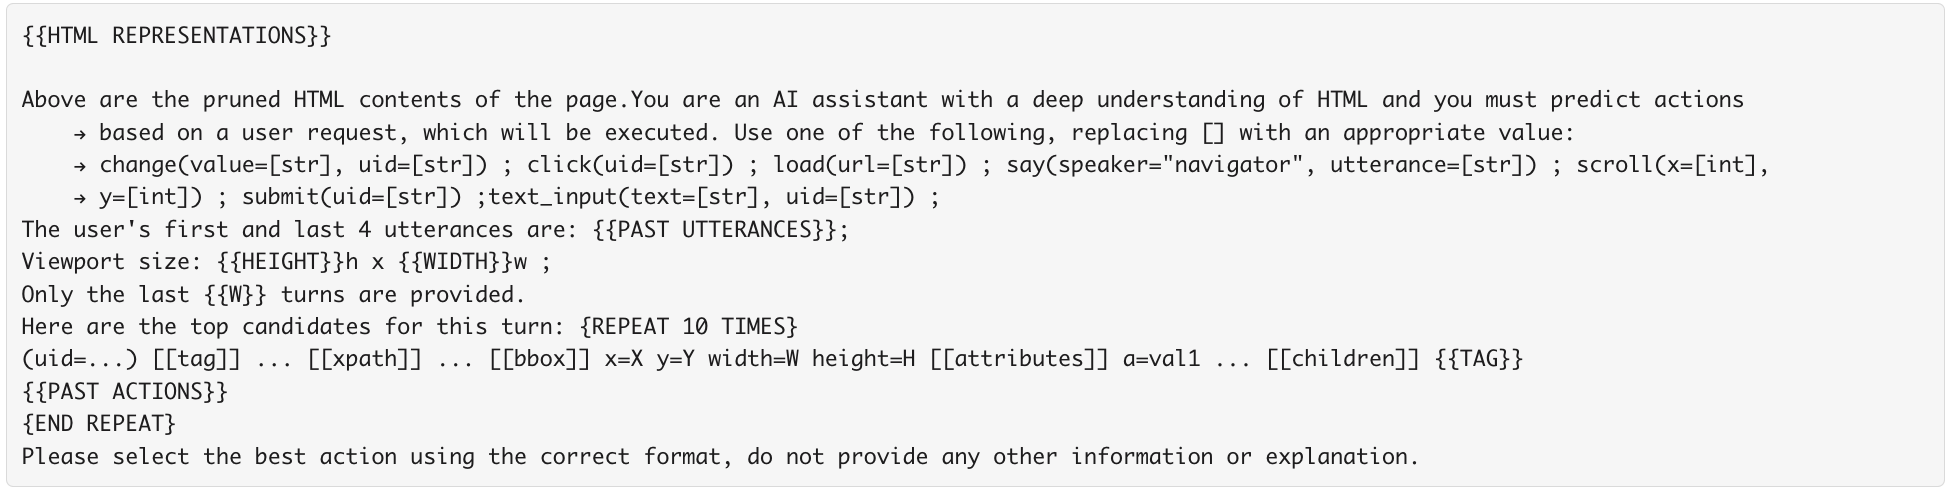
\includegraphics[width=\textwidth]{prompts/Chat-base-template.png}
\caption{Chat-based models baseline prompt template}\label{fig:fig1}
\centering
\end{figure}

\begin{figure}[ht]
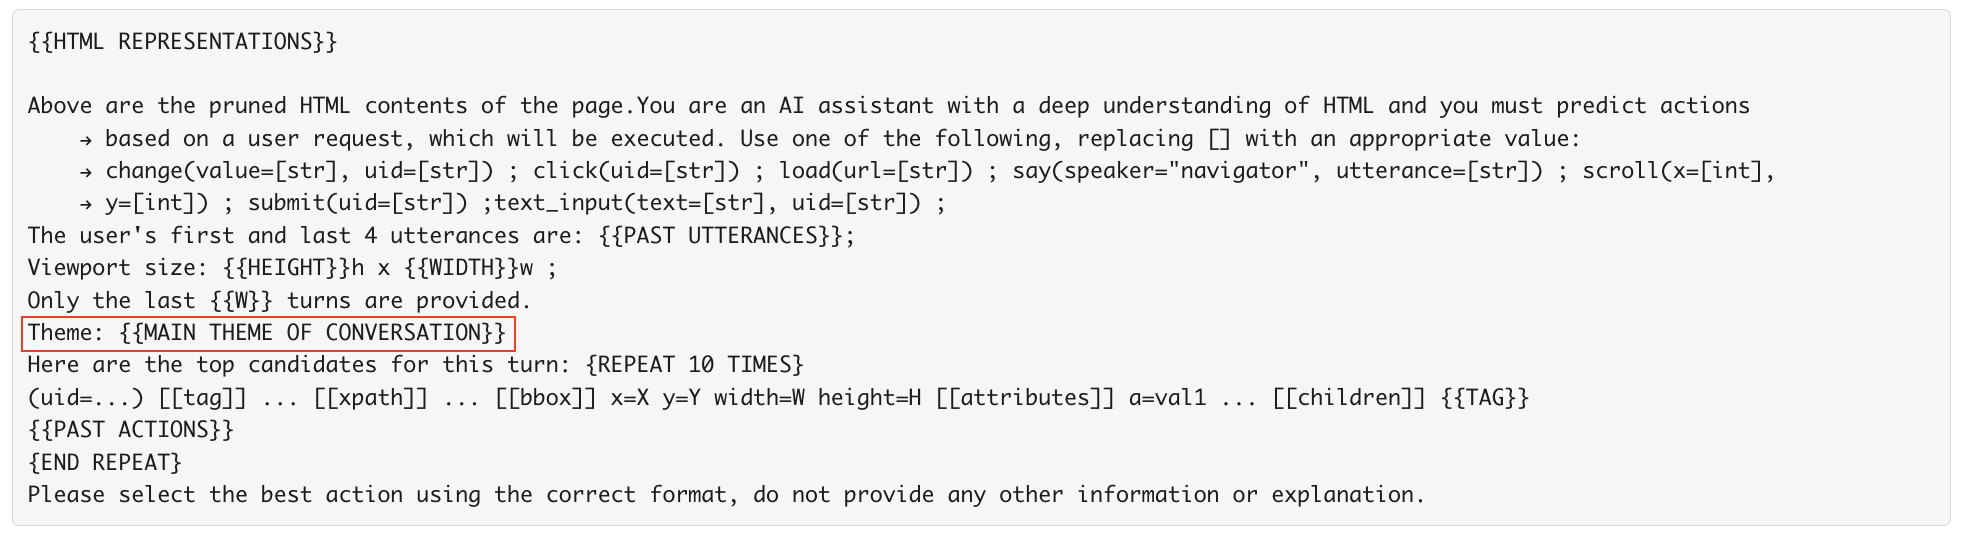
\includegraphics[width=\textwidth]{prompts/Chat-History-template.png}
\caption{Chat-based models prompt template with main theme of conversation included}\label{fig:fig2}
\centering
\end{figure}

\begin{figure}[ht]
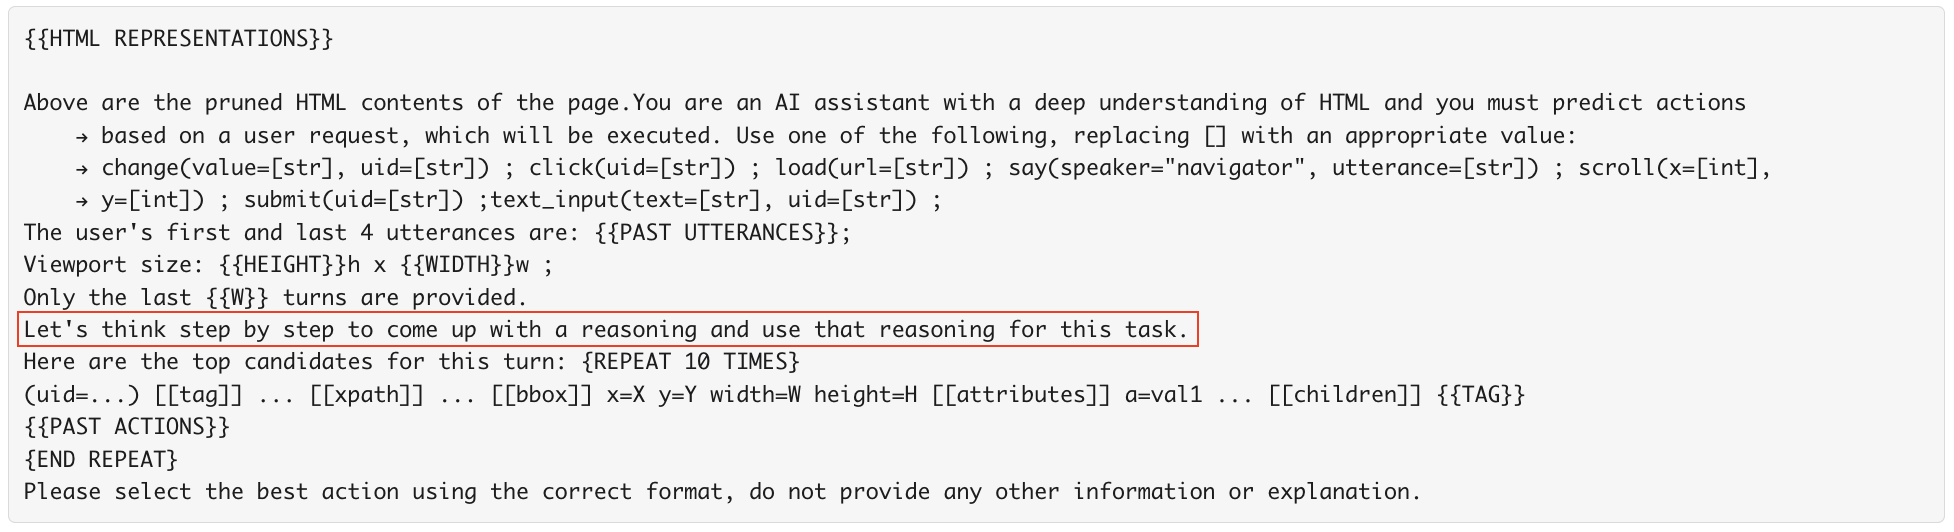
\includegraphics[width=\textwidth]{prompts/Chat-Zero-shot-template.png}
\caption{Chat-based models prompt template for zero-shot CoT}\label{fig:fig3}
\centering
\end{figure}

\begin{figure}[ht]
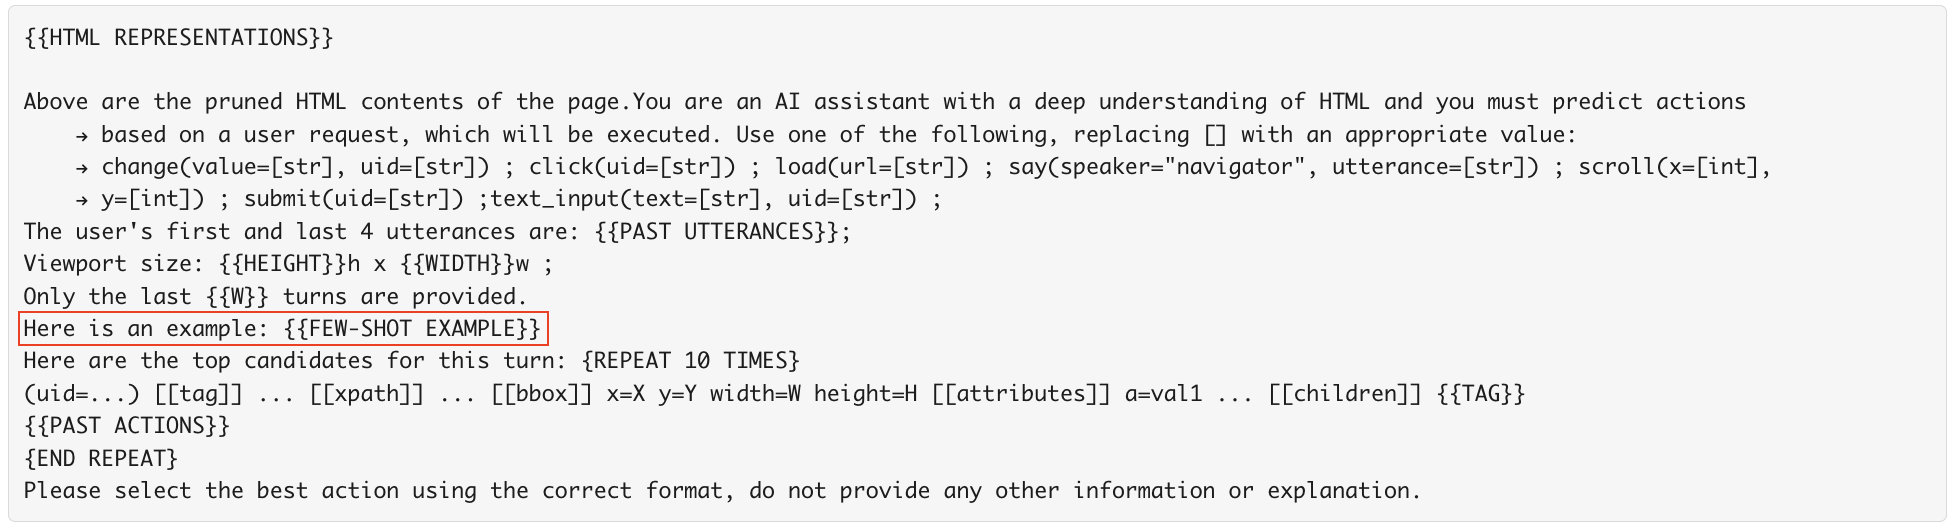
\includegraphics[width=\textwidth]{prompts/Chat-few-shot-template.png}
\caption{Chat-based models prompt template with few-shot CoT example}\label{fig:fig4}
\centering
\end{figure}

\clearpage

\subsection{Template Prompt for Instruction-based Models (Flan-T5)}

\begin{figure}[ht]
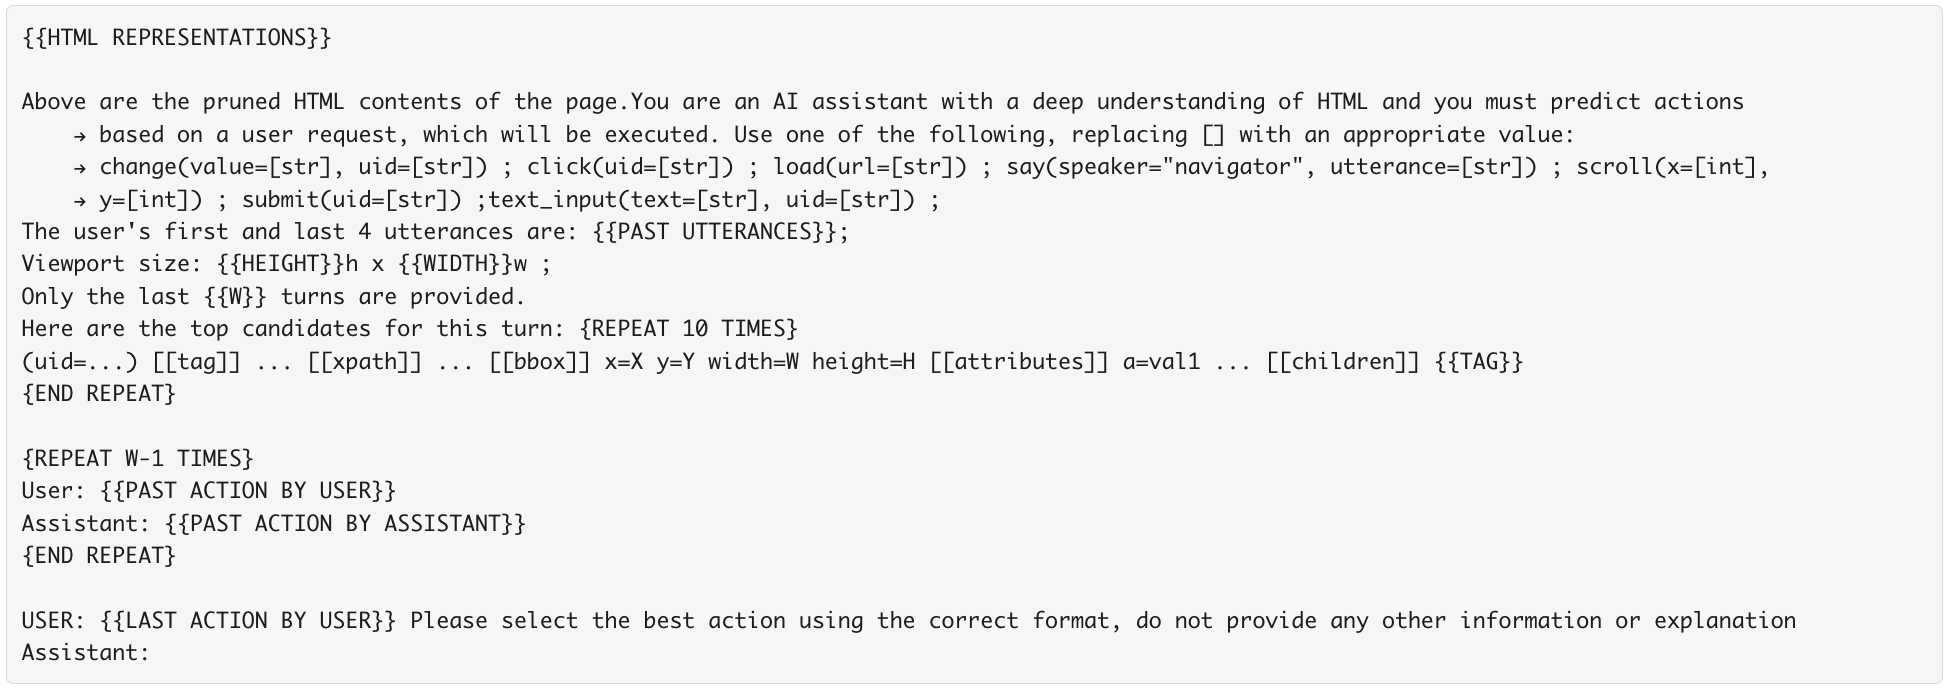
\includegraphics[width=\textwidth]{prompts/Instruct-base-template.png}
\caption{Instruction-based models baseline prompt template}\label{fig:fig5}
\centering
\end{figure}


\begin{figure}[ht]
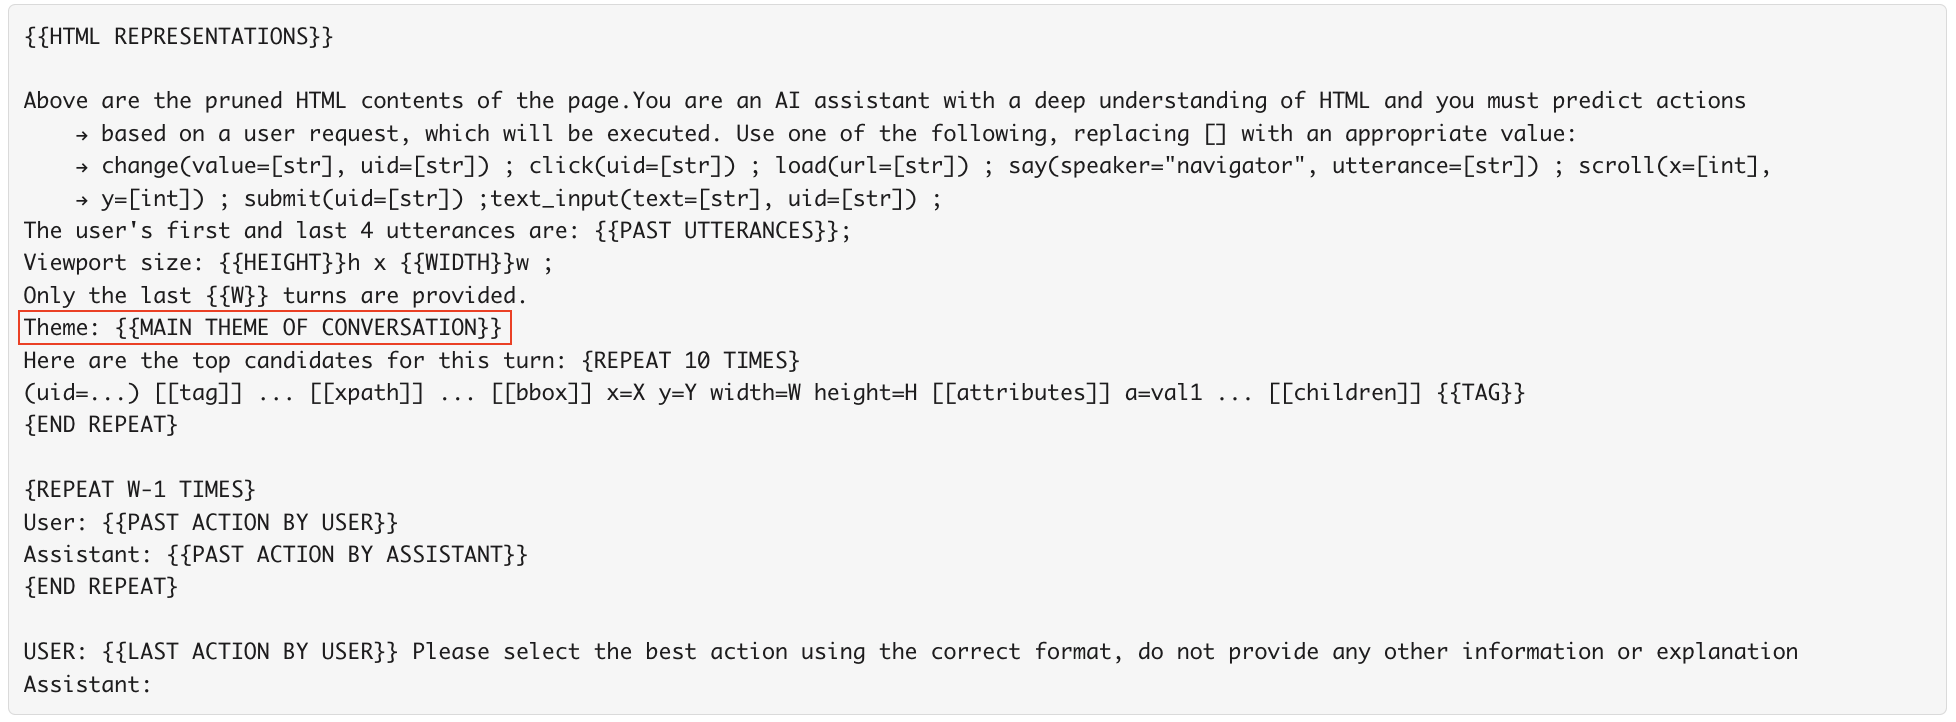
\includegraphics[width=\textwidth]{prompts/Instruct-history-template.png}
\caption{Instruction-based models prompt template with main theme of conversation included}\label{fig:fig6}
\centering
\end{figure}

\clearpage
\begin{figure}[ht]
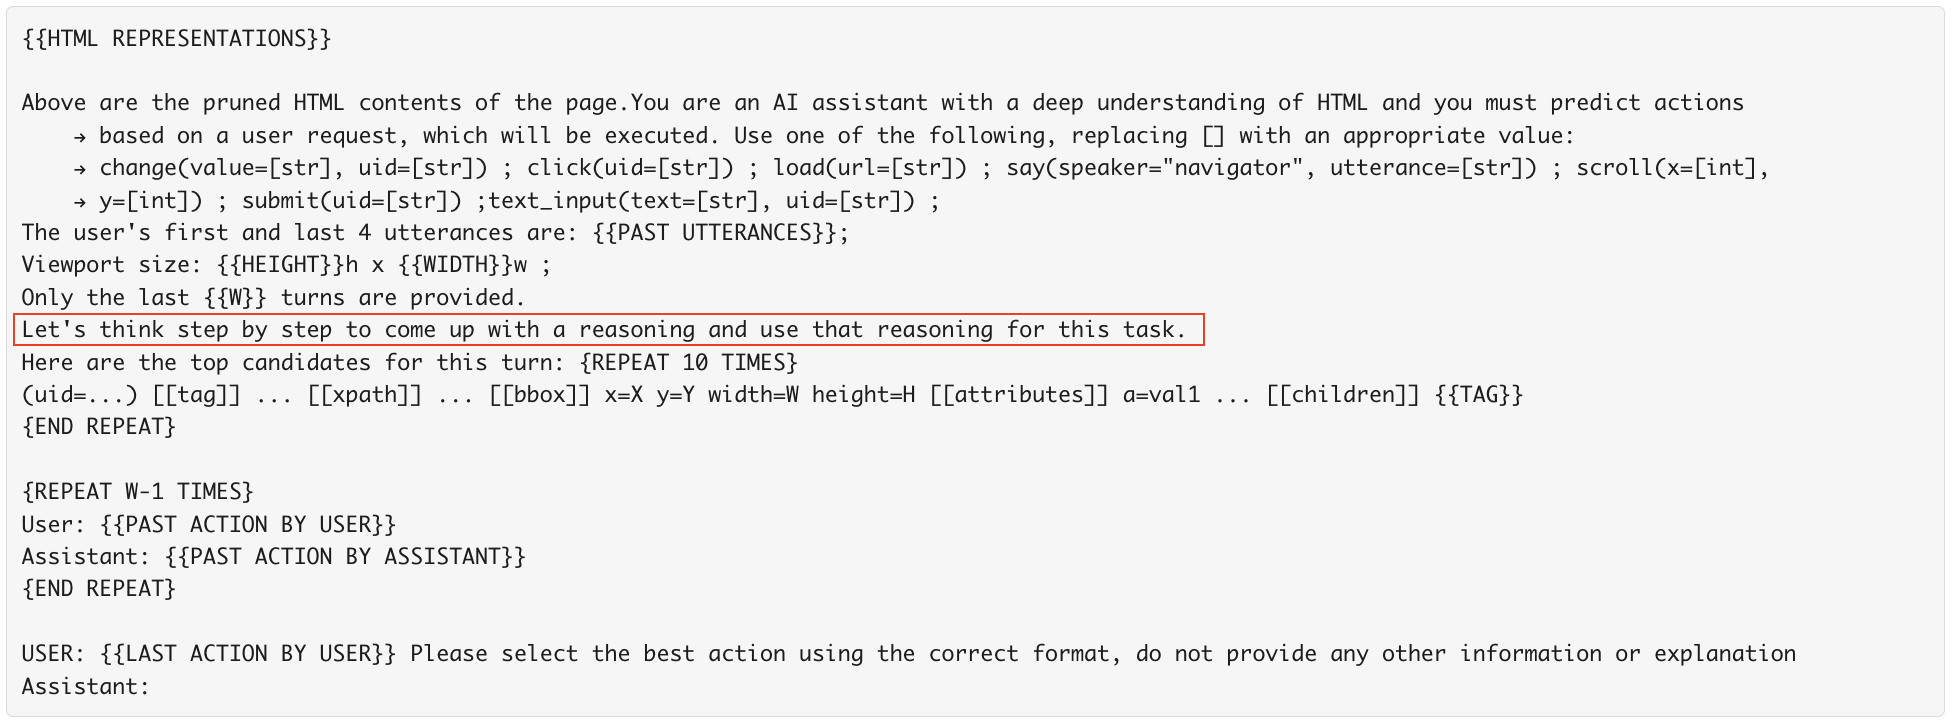
\includegraphics[width=\textwidth]{prompts/Instruct-zero-shot-template.png}
\caption{Instruction-based models prompt template for zero-shot CoT}\label{fig:fig7}
\centering
\end{figure}


\begin{figure}[ht]
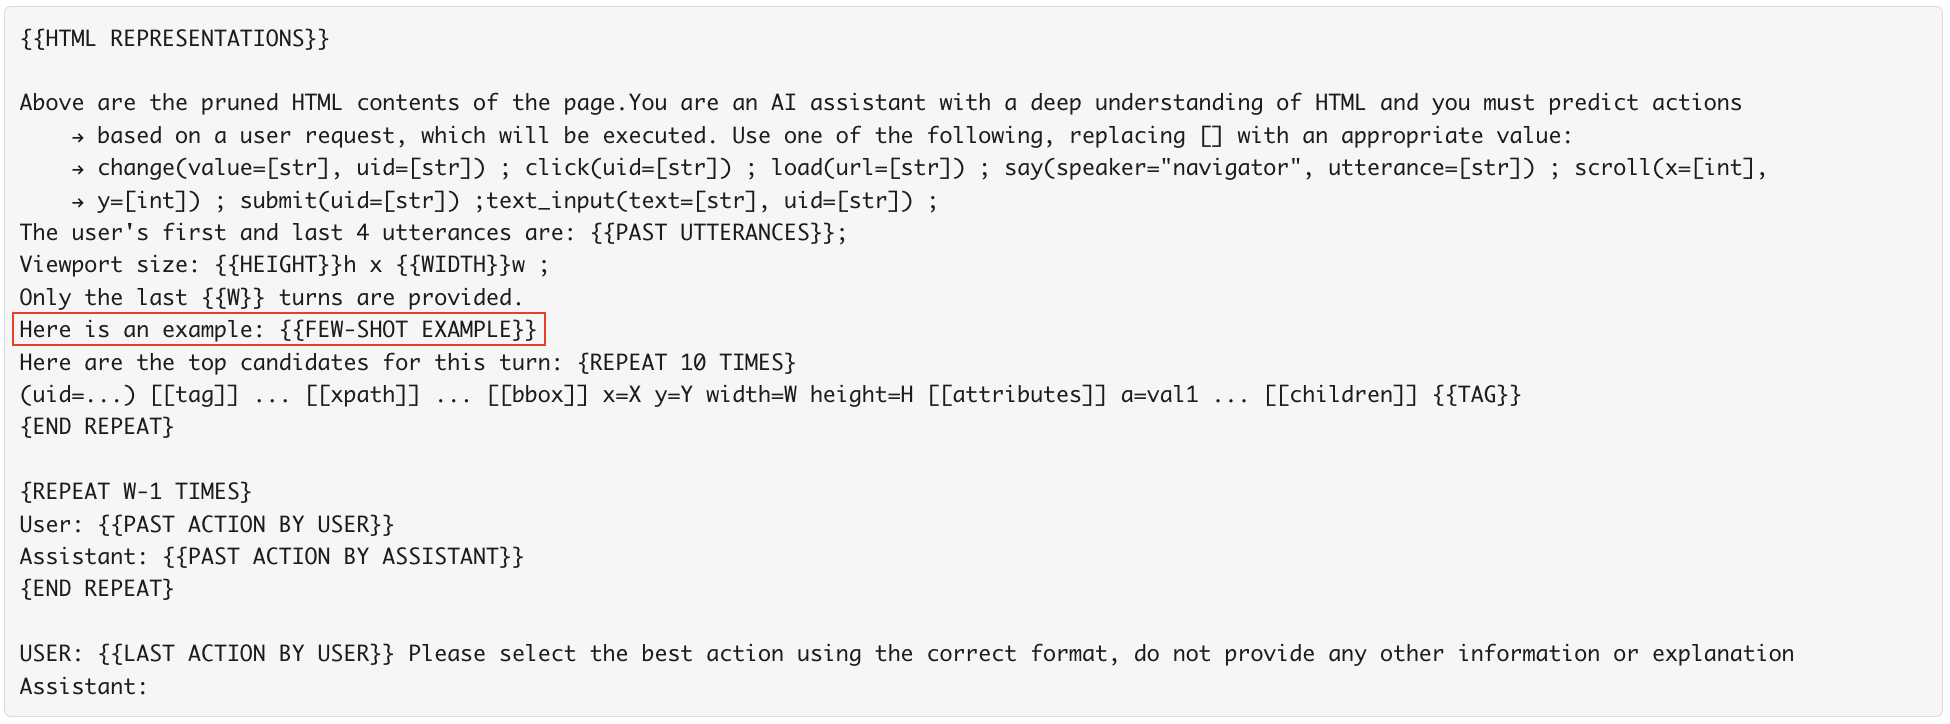
\includegraphics[width=\textwidth]{prompts/Instruct-few-shot-template.png}
\caption{Instruction-based models prompt template with few-shot CoT example}\label{fig:fig8}
\centering
\end{figure}

\section{Input Prompt Samples}\label{sec:samples}
We provide prompt samples for chat-based models like Sheared-LLaMA-1.3B and and for the instruction-based models like Flan-T5-780M. We show sample prompts for each of the three prompt experiments we conducted. 

\subsection{Sample Prompt Input for Chat-based Models (Sheared-LLaMA)}

\begin{figure}[ht]
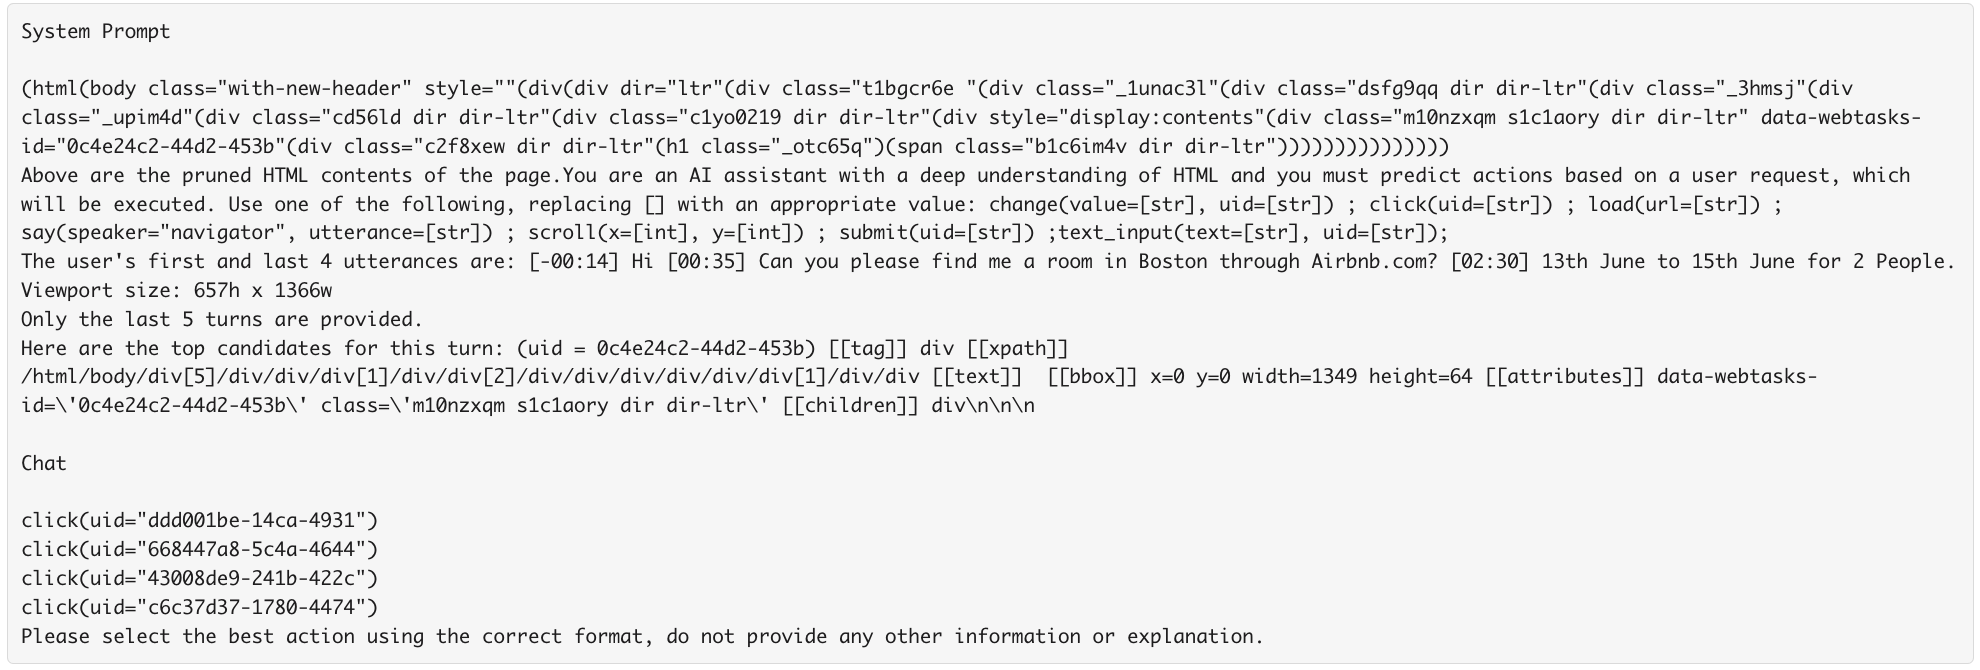
\includegraphics[width=\textwidth]{prompt_samples/Chat-base-sample.png}
\caption{Chat-based models baseline sample prompt}\label{fig:fig9}
\centering
\end{figure}

\begin{figure}[ht]
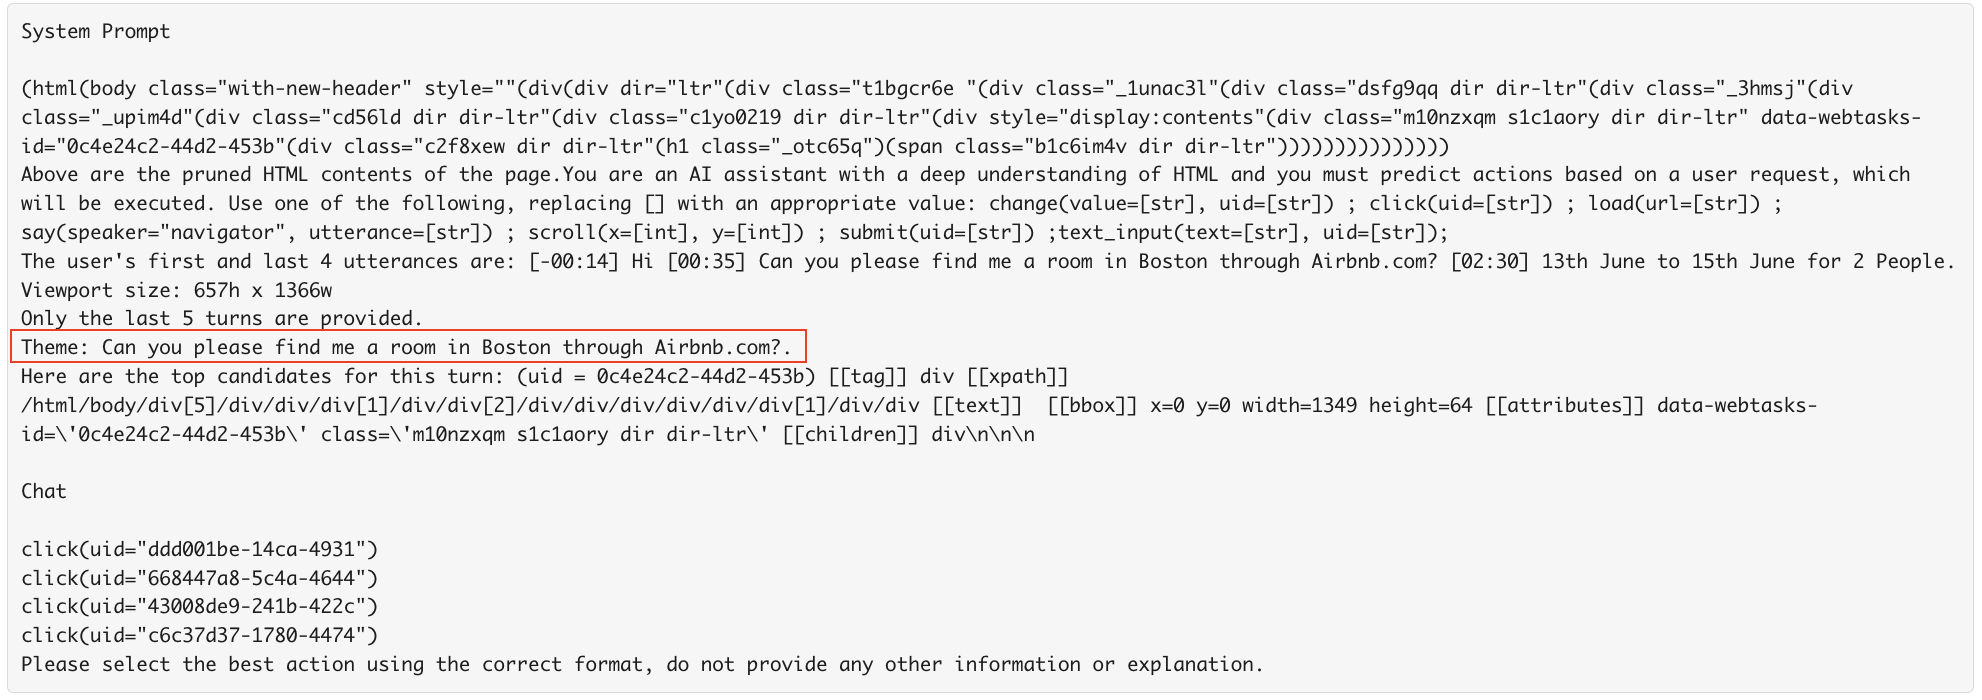
\includegraphics[width=\textwidth]{prompt_samples/Chat-History-sample.png}
\caption{Chat-based models sample prompt with main theme of conversation included}\label{fig:fig10}
\centering
\end{figure}

\clearpage
\begin{figure}[ht]
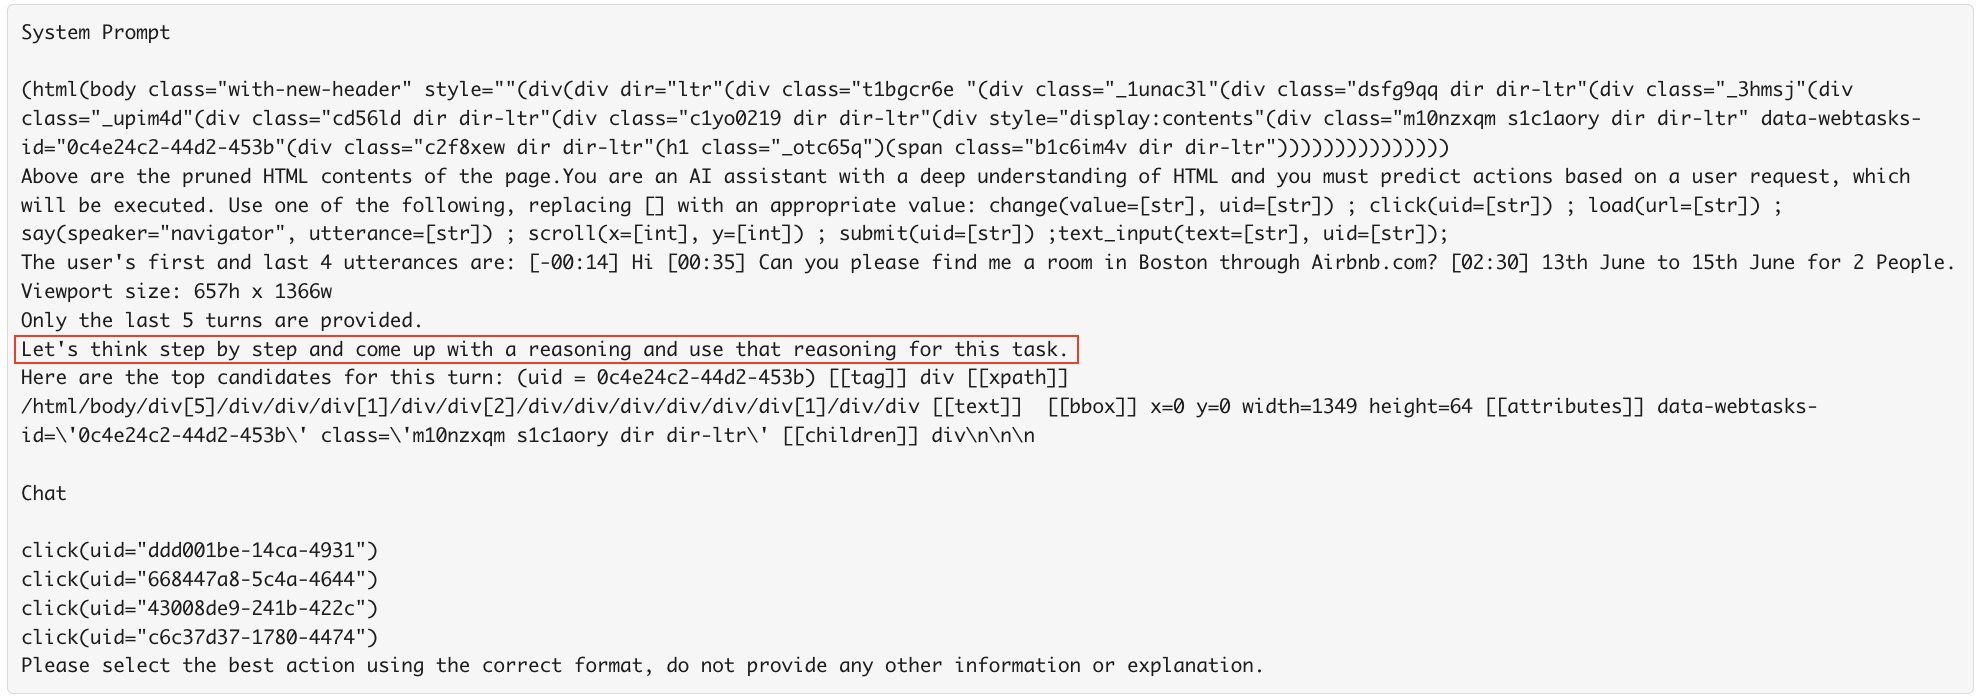
\includegraphics[width=\textwidth]{prompt_samples/Chat-zero-shot-sample.png}
\caption{Chat-based models sample prompt for zero-shot CoT}\label{fig:fig11}
\centering
\end{figure}

\begin{figure}[ht]
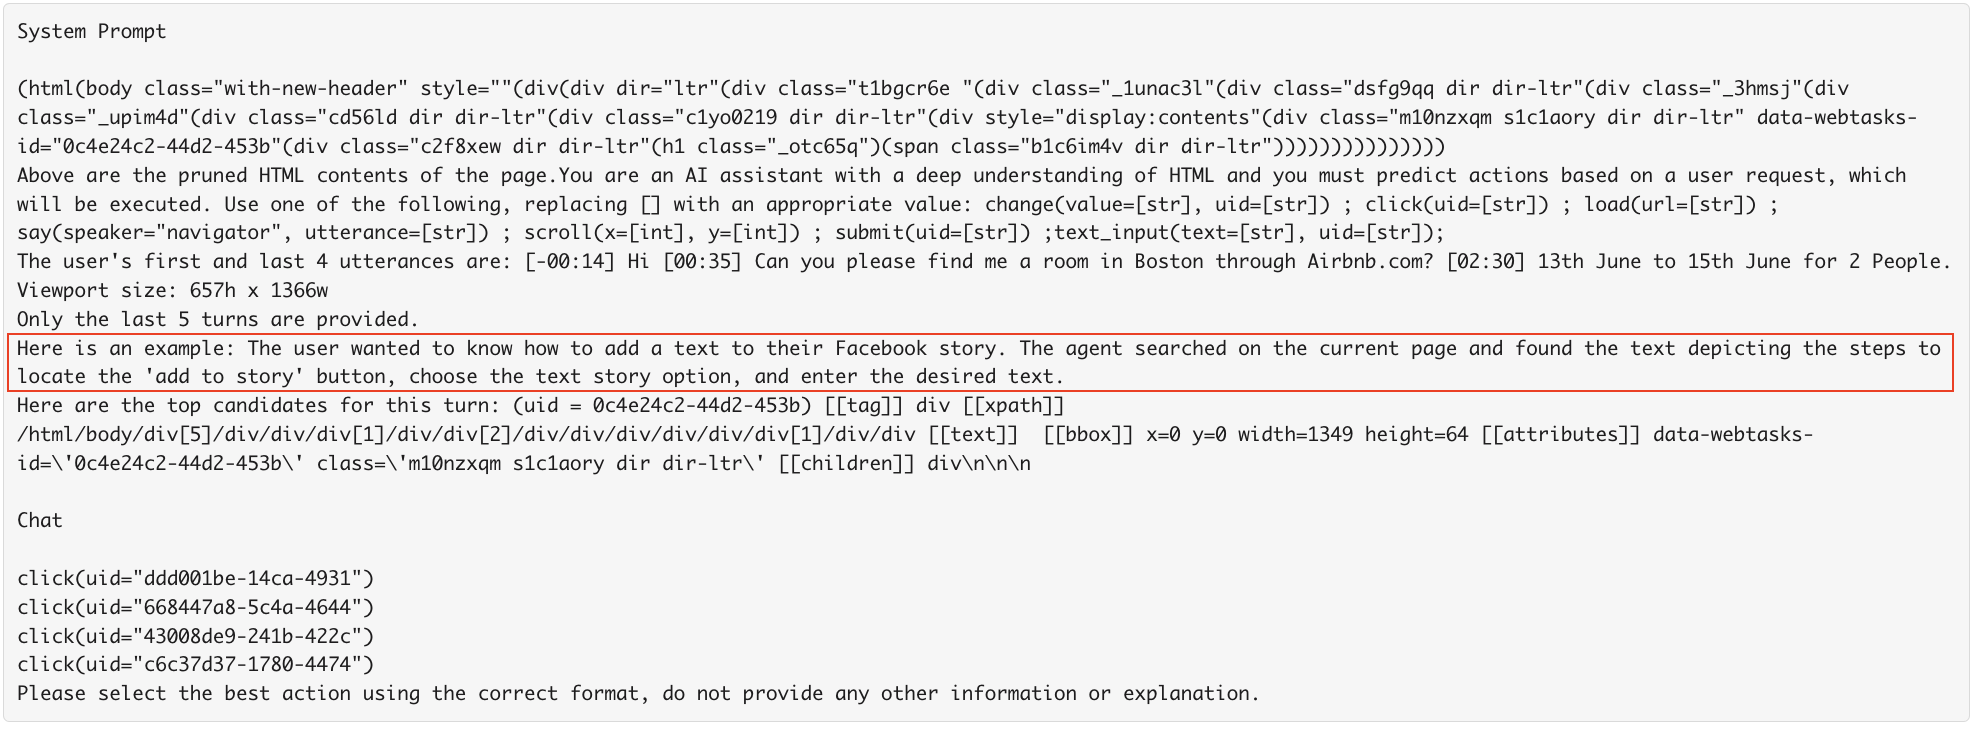
\includegraphics[width=\textwidth]{prompt_samples/Chat-few-shot-sample.png}
\caption{Chat-based models sample prompt with few-shot CoT example}\label{fig:fig12}
\centering
\end{figure}

\clearpage

\subsection{Sample Prompt Input for Instruction-based Models (Flan-T5)}

\begin{figure}[ht]
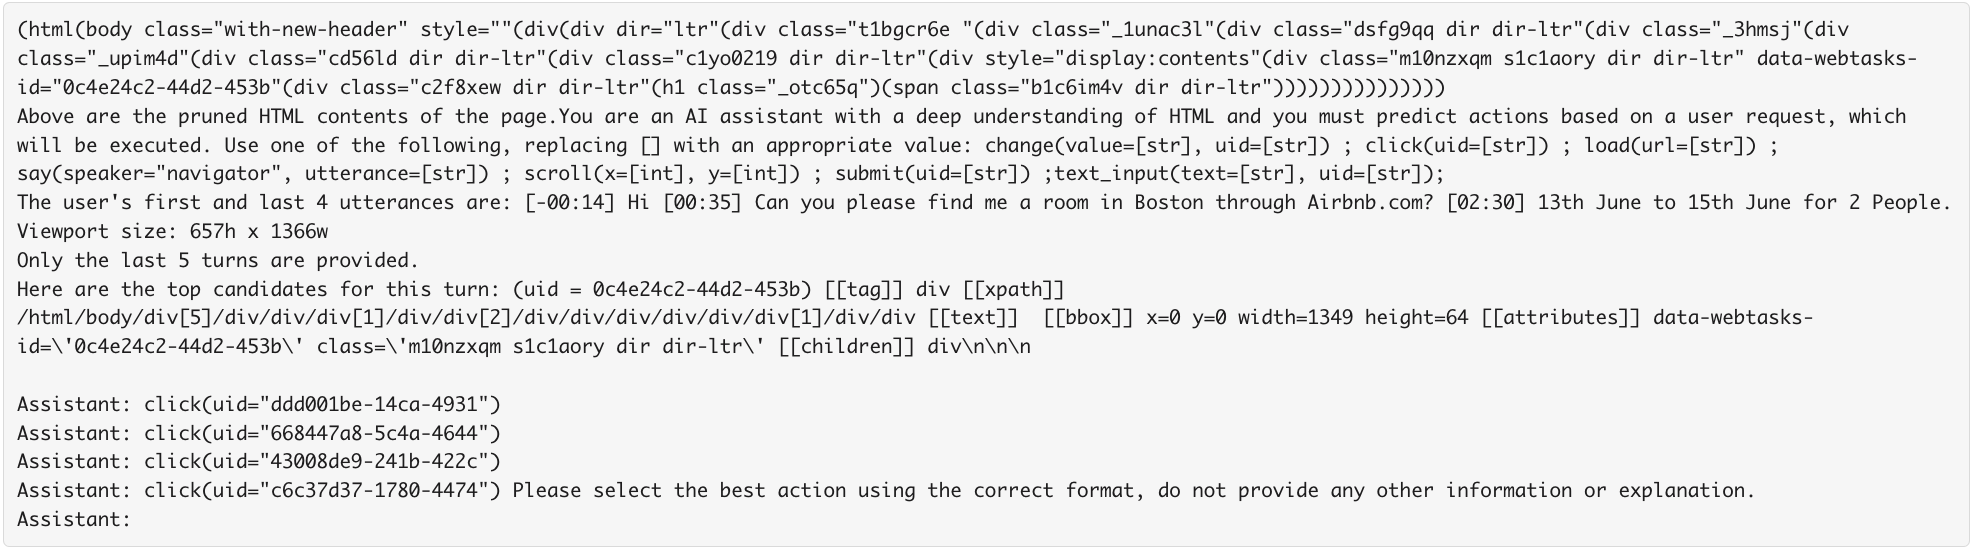
\includegraphics[width=\textwidth]{prompt_samples/Instruct-base-sample.png}
\caption{Instruction-based models baseline sample prompt}\label{fig:fig13}
\centering
\end{figure}
\begin{figure}[ht]
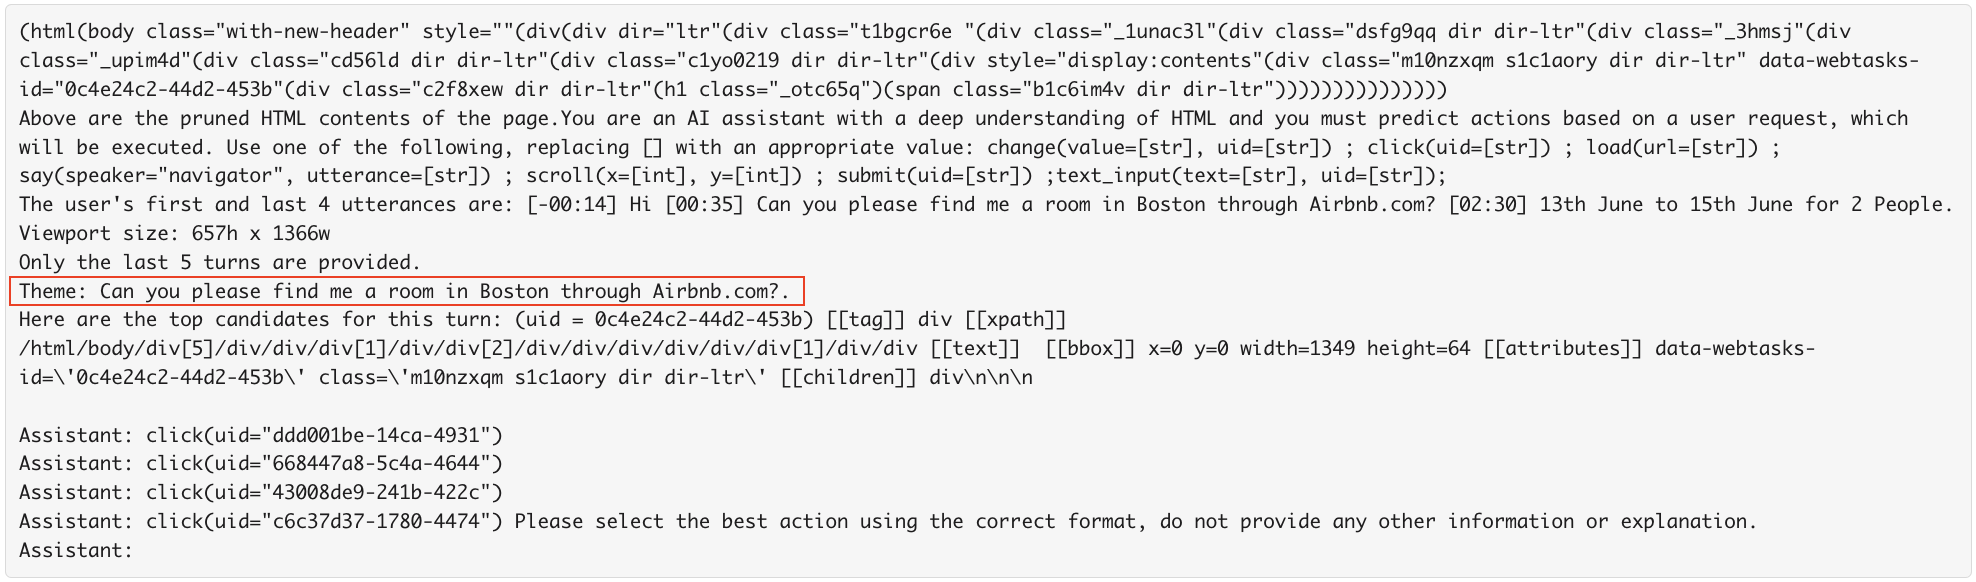
\includegraphics[width=\textwidth]{prompt_samples/Instruct-history-sample.png}
\caption{Instruction-based models sample prompt with main theme of conversation included} \label{fig:fig14}
\centering
\end{figure}
\begin{figure}[ht]
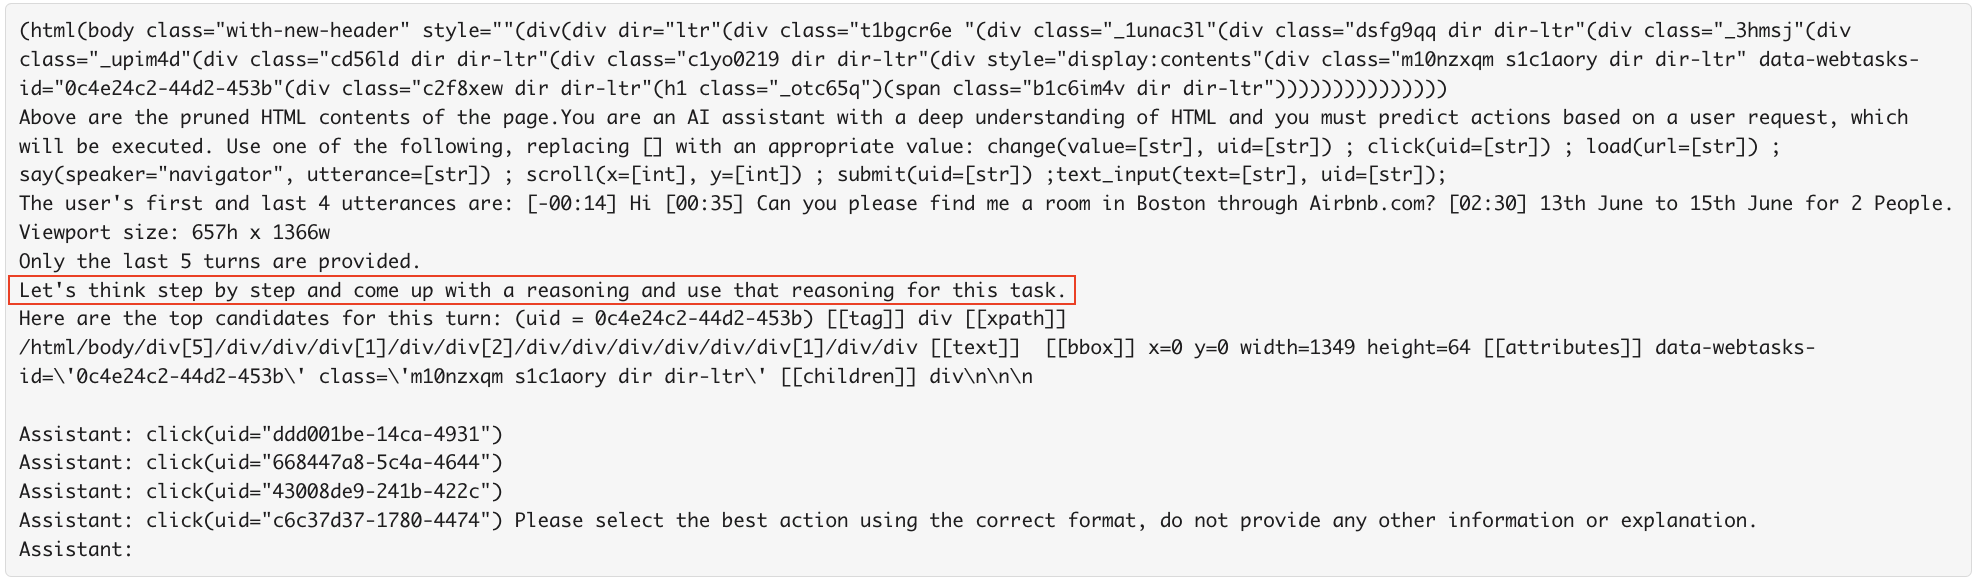
\includegraphics[width=\textwidth]{prompt_samples/Instruct-zero-shot-sample.png}
\caption{Instruction-based models sample prompt for zero-shot CoT} \label{fig:fig15}
\centering
\end{figure}

\clearpage
\begin{figure}[ht]
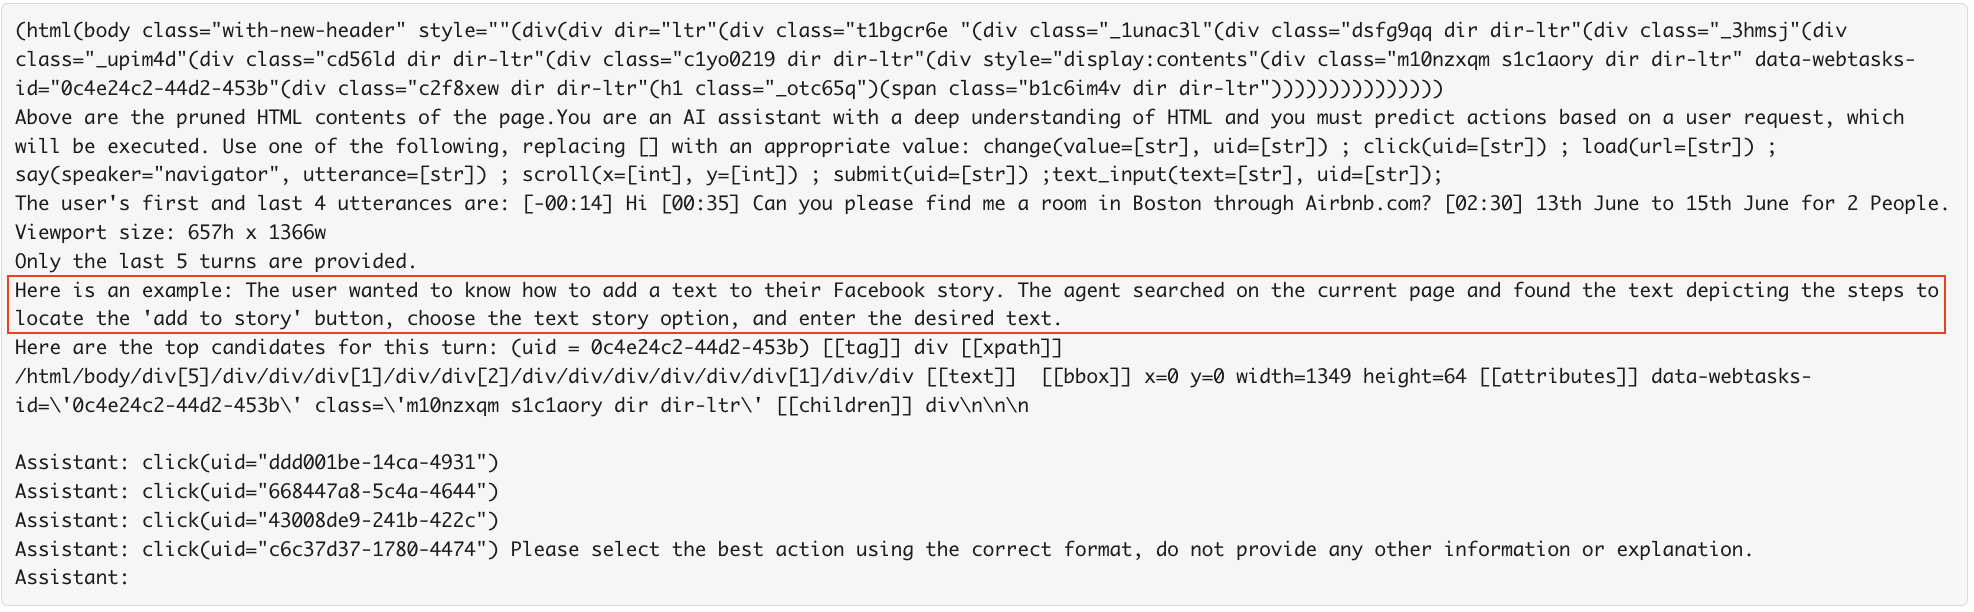
\includegraphics[width=\textwidth]{prompt_samples/Instruct-few-shot-sample.png}
\caption{Instruction-based models sample prompt with few-shot CoT example} \label{fig:fig16}
\centering
\end{figure}


\section{Summary of Other Exploratory Attempts}
\subsection{Training infra issues and setup}
\begin{itemize}
\item \emph{Dataset retrieval}:
Complete dataset download for WEBLINX was failing midway. It was tried about 10 times with the same issue. The job would stop while the download was in progress. The reason being there was no response from huggingface for the requested resource. We solved it by triaging the item for which this was occurring and manually downloading it. This needed to be done repeatedly across multiple jobs.
	\textbf{Error was: }\emph{raise HfHubHTTPError(str(e), response=response) from huggingface\_hub.utils.errors.HfHubHTTPError: 500 Server Error: Internal Server Error for url:  url\_omitted}

\item  The training performance was coming out to be too slow for the data-size we had. Managing data within the quota allocated on the home directory in Compute Canada and accessing it based on file permissions was problematic too.

\end{itemize}
    
\subsection{Embedding issue for multiple calls}
We were trying to use the \emph{MiniLM} model from SentenceTransformers to generate embeddings which we could use to pick the evolving main theme among the utterances. However, while trying to make it as part of the pipeline for building prompts, we were running into out of memory issues because the same object for the model was being passed to encode different dialogues across recursive calls. This made us go with a different approach to pick the main theme and we used the embeddings approach in a modular manner across single call separately.

\subsection{Explanation why we were not able to replicate baseline paper results} \label{sec:explanation}
We used regular floating point (FP16) during our evaluation instead of BF16 due to GPU compatibility issues. Both the models we used were of tensor type BF16. FP16 has 5 bits with the possible encoding range between $-65,000$ to $65,000$. Meanwhile BF16 can maintain the 32-bit number range, while having memory footprint similar to FP16. It can represent values up to $3.4$ x $10^{38}$. This means when we loaded the BF16 models using FP16, we would have lost the values by round off which were $>65,000$ or $<-65,000$. This means the model would have incurred some loss of information which might explain why we were not able to replicate the exact same values for the baselines.

\subsection{Experiments Details}
\begin{itemize}
    \item Hyperparameters: For each of the split we ran the evaluation, following parameters were maintained. The exhaustive list can be found in the github repository under config folder for the respective model. Top-10 candidates from the page were considered by the model to pick the next course of action. The batch size per device was set to 2.

    \item Software details: Due to dependency issues we encountered, we ended up using specific versions of the following packages to run our experiements. (torch==2.0.1 , datasets==2.14.0, cuda 11.7, huggingface-hub==0.17.0, tokenizers==0.14.1, transformers==4.35.0)
    
    \item Following modules were sideloaded on the compute canada cluster because we did not have sudo access on the nodes. (StdEnv/2020 gcc/9.3.0 arrow/13.0.0 rust/1.70.0 python/3.10.2 cudacore/.11.7.0)

    \item Implementation details: We used regular floating point instead of bf16 as used by the WEBLINX package. It would have led to increased memory usage but we did so because of dependency install issues.

    \item Our GPUs were not compatible with flash\_attention\_2. This would have led to reduced efficiency and longer execution times.

    \item Link to code repository : 
    \url{https://github.com/kpraays/PrompGent}
\end{itemize}

\end{document}
